% Created 2021-03-19 Fri 16:34
% Intended LaTeX compiler: pdflatex
\documentclass[a4paper,11pt]{article}
\usepackage[hyphens]{url}
\usepackage{float}
\usepackage[utf8]{inputenc}
\usepackage[T1]{fontenc}
\usepackage{graphicx}
\usepackage{grffile}
\usepackage{longtable}
\usepackage{wrapfig}
\usepackage{rotating}
\usepackage[normalem]{ulem}
\usepackage{amsmath}
\usepackage{textcomp}
\usepackage{amssymb}
\usepackage{capt-of}
\usepackage{hyperref}
\usepackage{rotating}
\usepackage[margin=1.25in]{geometry}
\usepackage{subfigure}
\usepackage{pdflscape}
\author{Tigany Zarrouk}
\date{\today}
\title{Atomistic investigation of dislocation-assisted carbon migration in iron}
\hypersetup{
 pdfauthor={Tigany Zarrouk},
 pdftitle={Atomistic investigation of dislocation-assisted carbon migration in iron},
 pdfkeywords={},
 pdfsubject={},
 pdfcreator={Emacs 27.1 (Org mode 9.4)}, 
 pdflang={English}}
\begin{document}

\maketitle
\tableofcontents

\clearpage

\begin{abstract}
Martensitic bearing steels have been shown to undergo subsurface microstructural decay, forming
Dark Etching Regions (DERs), promoting failure through rolling contact fatigue
(RCF). Dislocation-assisted carbon migration is thought to be the underlying mechanism, yet
empirical studies have been inconclusive as to how dislocations move carbon and where excess
carbon from the martensitic matrix migrates to upon transformation to ferrite---a phase of
significantly lower carbon solubility. In this report, we detail the first stage of a multi-scale
modelling approach to elucidate carbon transport by dislocations. Tight-binding simulations of
carbon interactions with the $1/2\langle 111 \rangle$ screw dislocation found solute distribution to vary
significantly within $\sim2$b of the easy and hard cores; the highest binding energy being found in
the centre of the hard screw core---which is the ground state carbon-dislocation
configuration---in agreement with Density Functional Theory (DFT). Determination of equilibrium
carbon concentration along dislocation lines, at various dislocation densities and nominal carbon
concentrations, found most sites around the hard core were saturated, with all easy cores
reconstructing to hard due to saturation of adjacent octahedral sites. In the typical temperature
range of bearing operation, we expect all dislocations to be of hard core type, pinned by carbon
in a prismatic site within the dislocation core. We anticipate large drag forces acting on
dislocations in the initial stages of glide, due to carbon-dislocation binding. These atomistic
results provide data for the last two stages in this multi-scale approach: determination
of kink-pair formation energies as a function of stress and carbon concentration using a line
tension model of a dislocation, and kinetic Monte Carlo (kMC) simulations incorporating solute
diffusion, to ascertain how carbon moves with dislocations in different stress, temperature and
concentration regimes.

\end{abstract}

\clearpage

\section{Introduction}
\label{sec:org2585bb1}

Martensitic steels are frequently used in bearings due to their resilience to service conditions,
being subject to high rotational speeds and contact pressures. However, under cyclic loading
exceeding a given contact stress, the microstructure of the steel can decay due to the accumulation
of plasticity. This signals the onset of rolling contact fatigue (RCF), which increases the risk of
failure from subsurface crack initiation. The microstructural decay corresponds to the observation
of Dark Etching Regions (DERs) as seen in optical microscopy, where the darkness of these regions is due
to the higher reactivity of DER phases to the etchant; exacerbated by
the roughness of the DER region \cite{skf2019}. See figure \ref{fuderpicture}.

\begin{figure}[htbp]
\centering
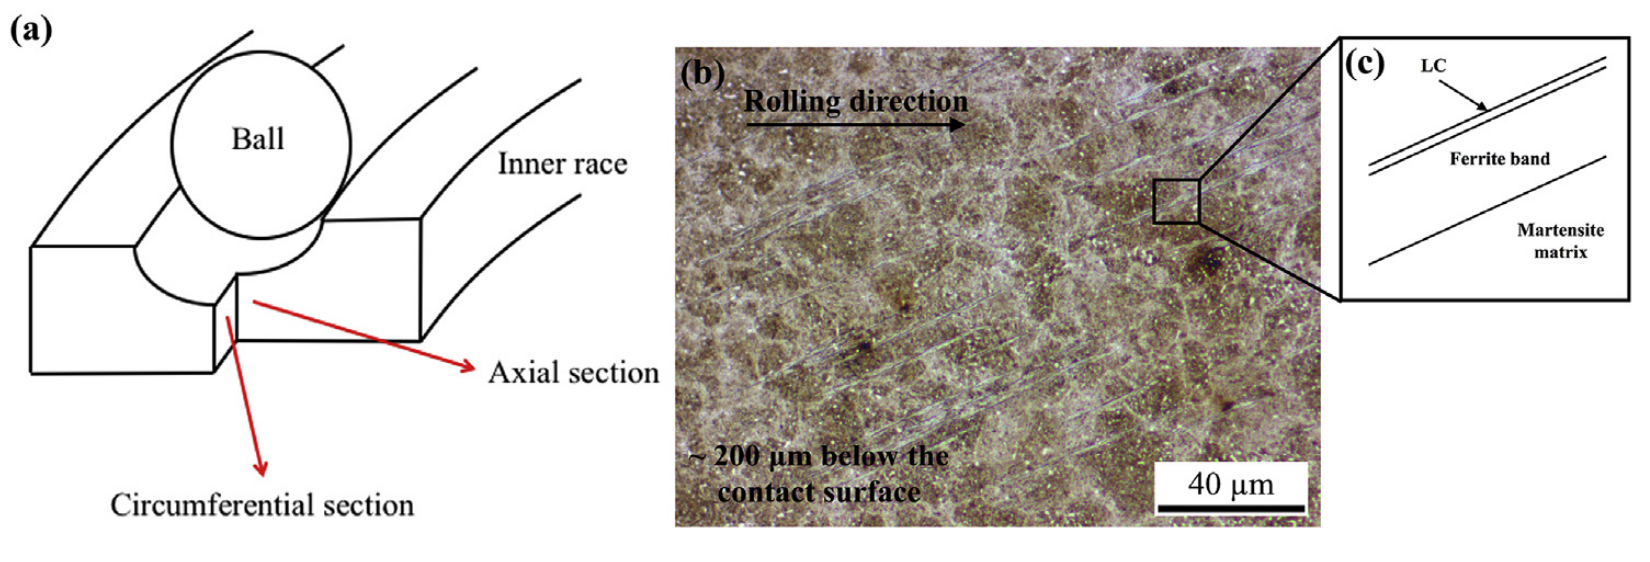
\includegraphics[width=.9\linewidth]{/home/tigany/Documents/docs/Management/Images/der_picture_fu.png}
\caption{Diagram of DER location within a bearing and its characteristics, taken from \cite{Fu2017}. (a) Axial and circumferential sections of a bearing inner ring. (b) Circumferential section of a bearing inner ring under optical microscope, where ferrite bands (white etching bands) are formed in the subsurface. (c) Diagram showing the structure of a WEB consisting of a ferrite band and a LC adjacent to it. One can see the DER region is composed of regions of ferrite interspersed in the parent martensite with lenticular carbides bordering the ferrite bands. \label{fuderpicture}}
\end{figure}


Decay of the martensitic microstructure is complex, with observation of many different
phenomena. Martensite transforms to ferrite microbands as a result of strain localization
\cite{Fu2017,il_micros_alter_rollin_contac_fatig,jonesil_metal_obser_ball_bearin_fatig_phenom,70_micros_microh_resid_stres_chang,Swahn1976,Voskamp1997,voskamp97_state_resid_stres_induc_by,polonsky95_white_etchin_band_format_rollin_bearin,vsmelova17_elect_micros_inves_micros_alter}. Residual
carbides, untouched at the start of DER formation, gradually dissolve within ferrite and
martensite \cite{70_micros_microh_resid_stres_chang,Swahn1976,Osterlund_1980}. Further RCF
progression leads to the formation of low and high angle ferrite features, White Etching Bands
(WEBs), composed of nanocrystalline \cite{Voskamp1997,Osterlund_1980,Mitamura_2007} and elongated
ferrite \cite{vsmelova17_elect_micros_inves_micros_alter}. Lenticular carbides precipitate at the
boundaries of these ferrite bands \cite{Swahn1976,Osterlund_1980}. Thickening of these carbides
occurs during DER development and is correlated with WEB growth
\cite{Fu2017,fu17_strain_induc_marten_decay_bearin,Warhadpande1_2013,Warhadpande2013}. Reductions in
dislocation density in nanocrystalline (heavily deformed) ferrite have been observed in the later
stages of DER formation \cite{skf2019,voskamp80_gradual_chang_resid_stres_micros}.



Carbon migration is thought to be the mechanism by which this degradation occurs, but it is not
definitively known how or where carbon migrates with the onset of DER formation. The key questions
are: where does excess carbon from the martensitic matrix find itself when the structure decays to
low solubility (0.02 wt\%) ferrite? and how is the carbon transported, given its low diffusivity in
martensite/DER phases
\cite{hashemi11_stren_hardn_statis_correl_api_x65_steel}? 


Fu \emph{et al.} propose that carbon atoms inside the martensite would segregate to
pre-existing/residual carbides, increasing their size
\cite{fu17_strain_induc_marten_decay_bearin}. This theory was successfully applied to the
growth of lenticular carbides \cite{Fu2017}, however, problems arise with the application to
temper carbide growth: if carbides were to form in martensite, they should follow the
Bagaryatskii/Isaichev orientation relationship, but observations suggest a lack of any orientation
relationship \cite{Bhadeshia2018}. Temper carbides residing within DERs have irregular
shapes/diffuse boundaries, which are seemingly due to the incomplete \emph{dissolution} of \emph{temper}
carbides, which is at odds with the theory of Fu \emph{et al.}.

A plausible mechanism for carbon migration is that it is driven by dislocation glide, which is as
follows
\cite{Fu2017,Swahn1976,voskamp97_state_resid_stres_induc_by,fu17_strain_induc_marten_decay_bearin,Warhadpande1_2013,Warhadpande2013}. Due
to the high dislocation density exhibited in martensite, carbon segregates to dislocations in
Cottrell atmospheres, causing pinning. Strain generated by cyclic stresses allow dislocations to
escape their carbon rich environment. The free dislocations re-attract carbon, allowing the
Cottrell atmospheres to reform, subsequently re-pinning the dislocations, creating a net carbon
flux.  This mechanism allows for the movement of carbon during the martensite-ferrite transition,
while also explaining how excess carbon can move from the ferrite phases to lenticular carbides at
the boundaries, describing the process behind both WEB growth and carbide thickening. Moreover, it
explains the dissolution of residual carbides, both in ferrite WEBs and martensite, due to
dislocation rearrangement and pile ups at the carbide interface drawing carbon atoms out, due to a
more favourable binding to dislocations. However, as to how this process occurs on the atomistic
scale, or if it is indeed feasible, is unknown.



Experimentally probing dislocation-assisted carbon migration has proven difficult and inconclusive. Work needs to be done
to understand dislocation-carbon interactions; more specifically: how dislocations move carbon
within the temperature and stress regimes experienced during operation; where carbon is
transported to and what the resultant dislocation networks are. 


To shed light on this mechanism, a multi-scale modelling approach can be
used. Atomistics can provide information of the 2d Peierls energy landscape which dislocations are
subject to in iron; and how this landscape is modified by the binding of carbon to
dislocations. This data can be used in a line tension model of a dislocation to determine the
kink-pair formation energies of dislocations as a function of carbon content and stress. Finally,
one can use a kinetic Monte Carlo (kMC) model of dislocation glide by thermally activated
kink-pair nucleation, in an environment of carbon. From this last stage of coarse-graining, one
can determine in which regimes of temperature, stress and carbon concentration,
dislocation-assisted carbon migration becomes a feasible mechanism behind DER formation, with
predictions of dislocation velocity, dislocation configurations and where carbon moves with
dislocation glide. 

In this report, we will focus on the atomistic portion of this project,
directed at understanding dislocation-carbon interactions at the atomistic scale in ferrite (bcc
iron).
With further knowledge of the fundamental mechanism behind DER formation, we can hope to suppress
dislocation motion in the martensitic matrix, mitigating failure by RCF.



\section{Computational Method}
\label{sec:org3bb57cb}


We use the tight-binding model of Paxton and Elsässer \cite{Paxton2013}, which has been shown to
describe the binding energies of carbon complexes in bcc iron, in good agreement with DFT
calculations. This model reproduces the two screw dislocation core structures---the easy and hard
\(1/2\langle 111 \rangle\) cores---exhibited in bcc iron. Study of both is crucial to understanding
solute-dislocation interactions. The easy core is the ground state in pure iron, but solutes, such
as hydrogen and carbon, have been shown to reconstruct this core into the hard core
configuration \cite{Ventelon2015,itakura13_effec_hydrog_atoms_screw_disloc}. Computationally cheaper
models, which do not incorporate quantum mechanics, such as the EAM, cannot reproduce these
behaviours.


\subsection{Peierls Potential}
\label{sec:org54e9df0}

To determine the Peierls potential of the \(1/2\langle 111 \rangle\) screw dislocation, we followed the
procedure detailed in Itakura \cite{Itakura2012}. Quadrupolar arrays of dislocations were
constructed by placing dislocations of antiparallel \(1/2\langle 111\rangle\) Burgers vectors in an "S"
arrangement \cite{Clouet2012}, with initial displacements determined by anisotropic elasticity
solutions. See figure \ref{fig:dislocationschematics}, left. A quadrupolar arrangement minimises
the stress each dislocation experiences in the simulation. These displacements were modified to
be periodic, thereby removing artificial stacking faults which would appear between periodic
images after introduction of the dislocation dipole. This was achieved by the subtraction of a
linear error term from the superposition of displacement fields arising from the dislocations in
the simulation cell and its periodic images \cite{vasilybulatov2006}. To accommodate for the
internal stress upon introduction of a dislocation dipole into the simulation cell, an elastic
strain was applied to the cell, resulting in an additional tilt component to cell vectors
\cite{Clouet2012,vasilybulatov2006,Clouet2009}. Simulation cells were constructed with different initial core
positions, which were sampled from the triangular region "EHS" (easy, hard and split) core
positions, as detailed in figure \ref{sampledpositions}. To fix the dislocation positions during
relaxation, the three atoms surrounding the easy core, for each dislocation, were fixed in \(Z\)
coordinate during relaxation, where \(Z\) is a \(\langle 111 \rangle\) direction, along the dislocation line. The
k-point sampling mesh for each of these cells was 5x5x30.


        \begin{figure}
    \begin{tabular}{cc}
	     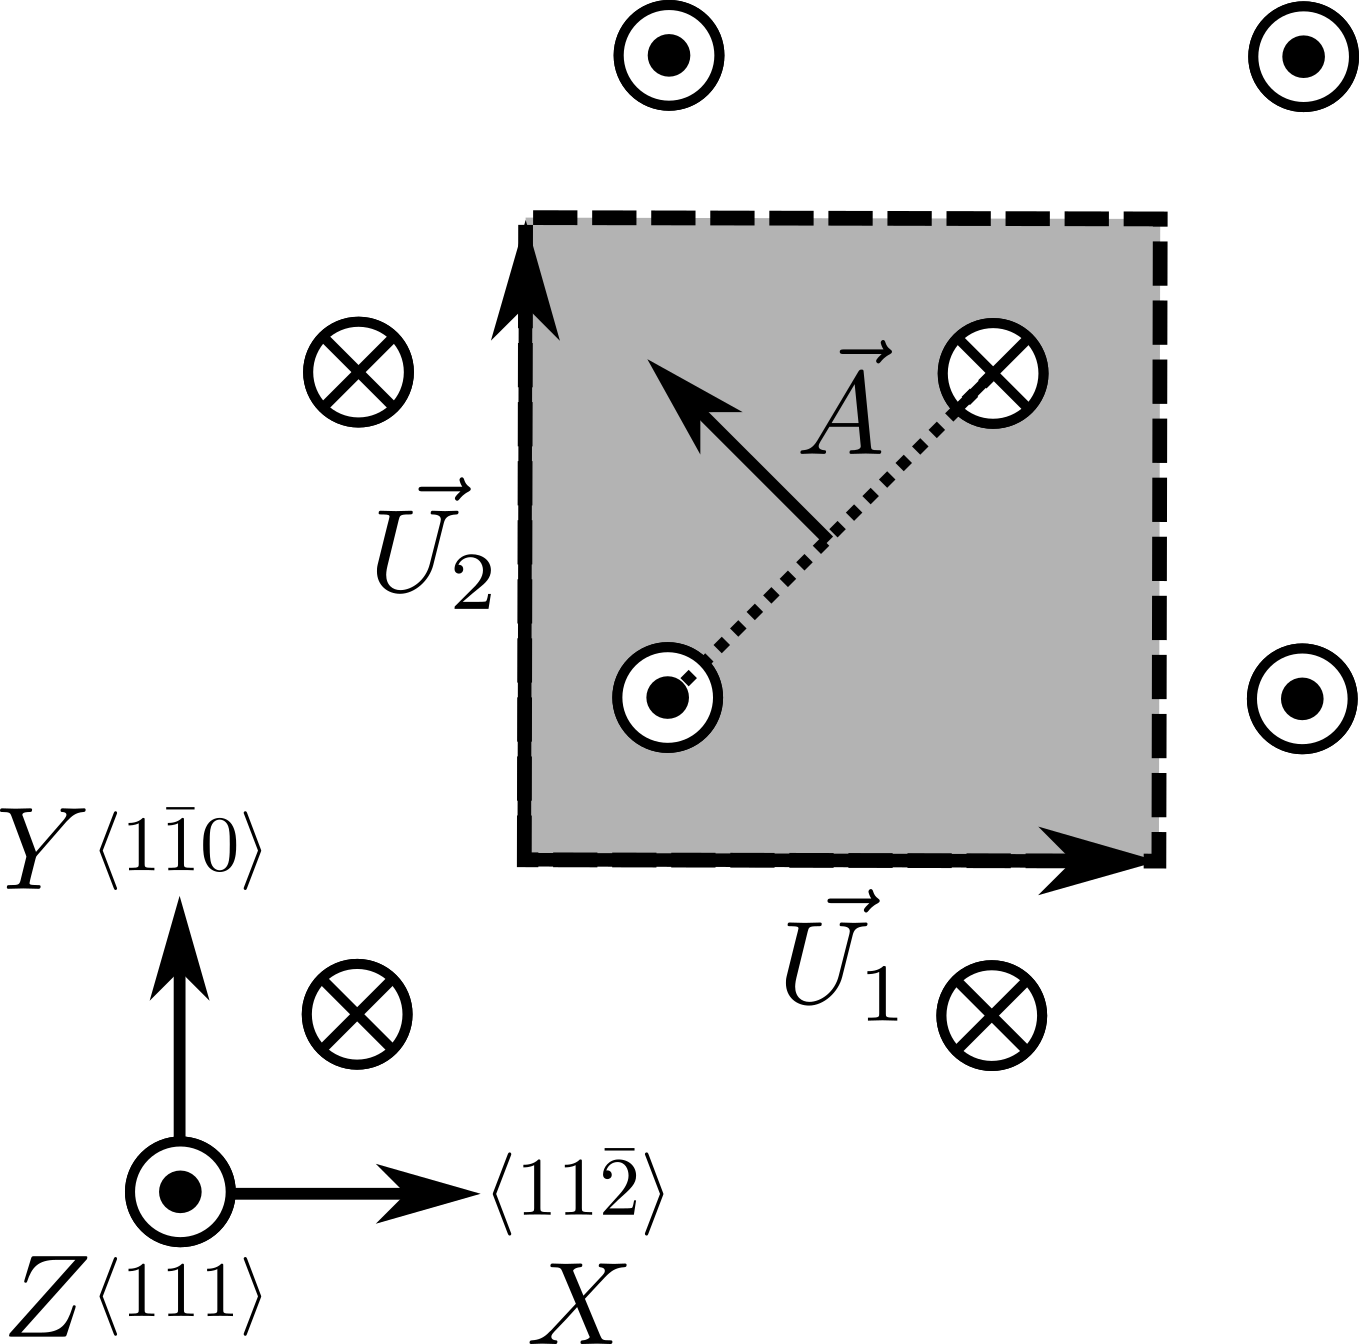
\includegraphics[width=0.5\textwidth]{Images/s_arrangement_quadrupole.png} &
             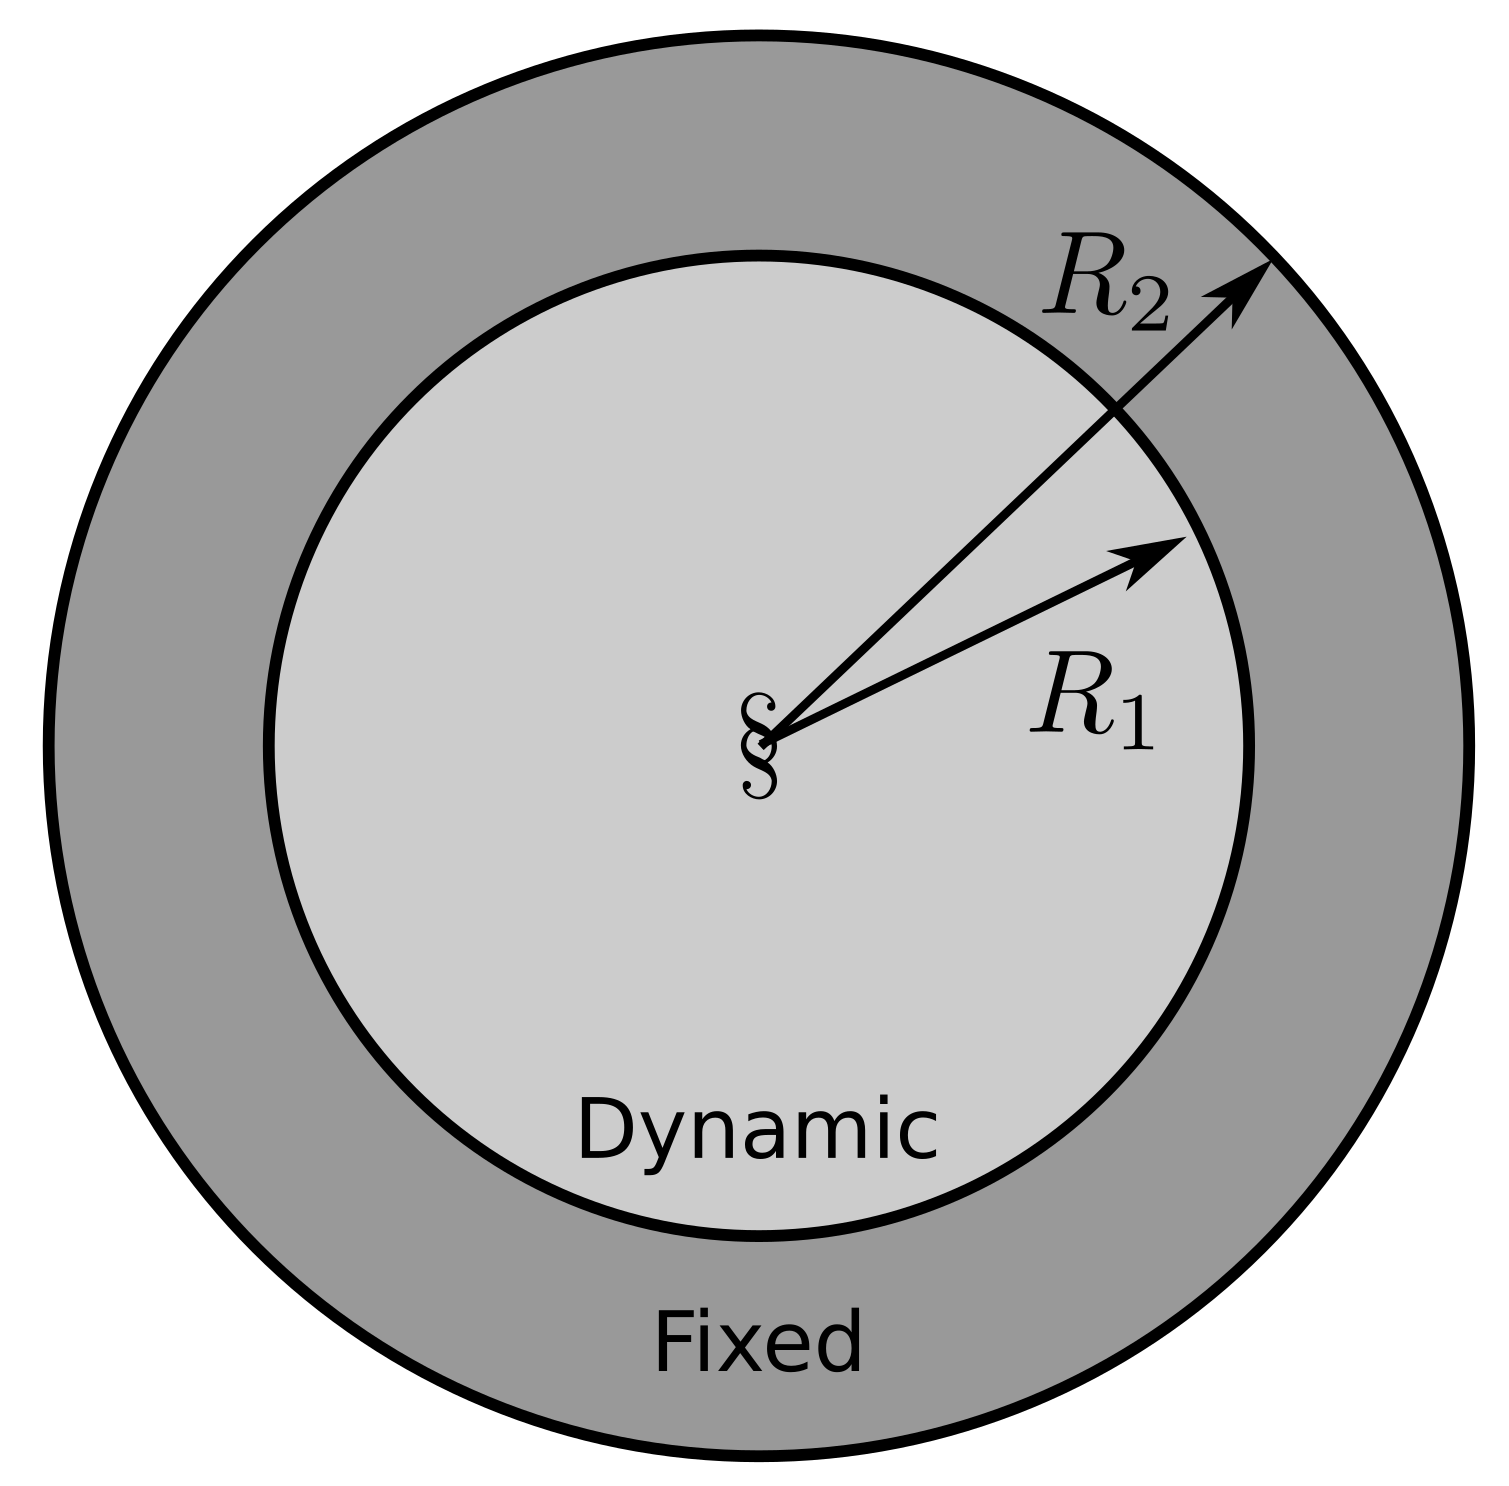
\includegraphics[width=0.45\textwidth]{Images/cluster_method_schematic.png}  \\
    \end{tabular}		
\caption{Schematics of dislocation simulation methods. Left: quadrupolar arrangement of dislocations in a simulation cell (grey square). This arrangement  minimises the stress experienced by each dislocation in a periodic simulation. Cell vectors $\vec{U}_1$ and $\vec{U}_2$ are shown; $\vec{A}$ defines the cut plane between the dipoles. The dislocation positions, and their corresponding burger's vector direction, are denoted by the symbols $\otimes$ and $\odot$, which are antiparallel to each other. Tilt components added to cell vectors to accomodate for the plastic strain are not shown. Right: cluster method, where atoms are displaced according the displacement field from the screw dislocation at the centre of the cluster, denoted by "\S". Atoms in the annulus $R_2 - R_1$ are fixed in position to the anisotropic elasticity solutions. Within $R_1$, all atoms can relax. Periodicity is only imposed in the $Z$ direction.}
	\label{fig:dislocationschematics}
    \end{figure}



        \begin{figure}
    \begin{tabular}{cc}
	     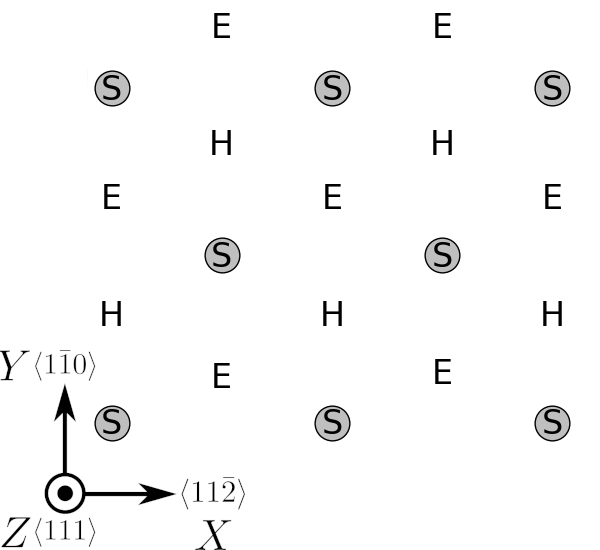
\includegraphics[width=0.5\textwidth]{Images/hardeasycoreatomdiagram_coordnew.png} &
             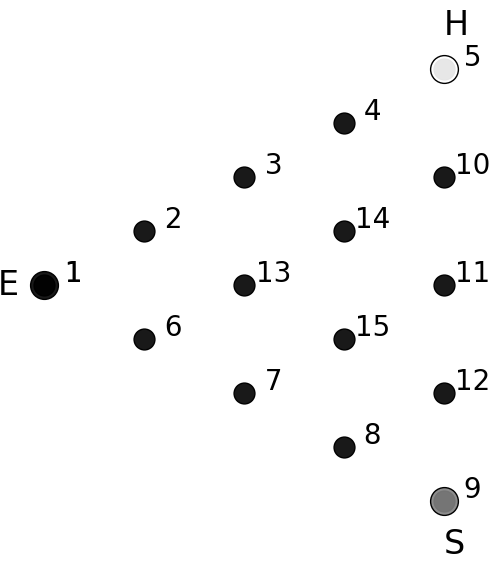
\includegraphics[width=0.45\textwidth]{Images/peierls_potential_positions_tbe.png}  \\
    \end{tabular}		
\caption{Diagrams of dislocation core positions. "E", "H" and "S" correspond to the easy, hard and split core positions respectively. Left: core positions as seen along the $Z=\langle 111 \rangle$ direction, along the dislocation line. Atomic positions are shown as grey circles. Right: positions sampled within the triangle EHS used to determine the Peierls potential.  \label{sampledpositions}}
	\label{fig:peierlspot}
    \end{figure}


The interaction energy between the dislocation dipole and periodic images was defined differently
to Itakura \cite{Itakura2012}. We followed the prescription of Bulatov and Cai \cite{vasilybulatov2006} to
find a regularised interaction energy, which is independent of truncation limit, in contrast to
the formulas quoted in Itakura's papers. Details can be found in section \ref{sec:Ainteractionenergy}.




The Peierls potential \(\Delta E_{\text{P}}^i\), for an isolated dislocation at the \(i^{\text{th}}\) core
position, can be calculated from
\begin{equation}
 \Delta E_{\text{P}}^i = \Delta E_{\text{tbe}}^{i} - \Delta E_{\text{INT}}^{i} ,\label{eq:peierlspot} 
 \end{equation} 
where \(\Delta\) refers to quantities, per dislocation, relative to the relaxed easy core configuration
(labelled as E/1, as in figure \ref{sampledpositions}). \emph{e.g} \(\Delta E_{\text{tbe}}^{i} = \frac{1}{2} (
   E_{\text{tbe}}^{i} - E_{\text{tbe}}^{\text{E}} )\) is the difference in energy, per dislocation, between
a relaxed cell which has the two dislocation cores placed at position \(i\), \(E_{\text{tbe}}^{i}\), and a relaxed
cell which has the two cores placed in easy core positions \(E_{\text{tbe}}^{\text{E}}\), divided by the number of
dislocations in each of the simulation cells. Dislocation-dislocation interaction
energies are included in this term, due to dislocations in the simulation cell---and
periodic images---interacting with each other, as can be readily seen in figure
\ref{fig:dislocationschematics}. To model the energy landscape of an isolated dislocation, these
interaction energies must be subracted, which is achieved by the correction term \(\Delta E_{\text{INT}}^{i}
   = \frac{1}{2} ( E_{\text{INT}}^{i} - E_{\text{INT}}^{\text{E}} )\).

\subsection{Preliminary calculations}
\label{sec:org3530295}
To determine the binding energy of carbon to dislocations, we used the cluster method, as shown
in figure \ref{fig:dislocationschematics}, right. Simulation
cells consisted of a cylindrical cluster of atoms, with a single dislocation introduced into the
centre using displacements from anisotropic elasticity solutions. Each of the clusters were
centred on the easy or hard core positions. The cluster of atoms was split into two regions: a
central region of dynamic atoms with radius \(R_1\), and an annulus of atoms, between \(R_1\) and \(R_2\),
which were fixed in position to the displacements from anisotropic elasticity.


To confirm the anisotropic elasticity solutions were correct, we compared the
displacements against the analytic solutions to the straight screw dislocation, as given in Hirth
and Lothe \cite{Anderson2017}. Furthermore, energy scaling relations were verified. We
inserted dislocations into cells of varying radii: \(R_1 = x\sqrt{2}a_{\text{bcc}}\), and \(R_2 =
   (x+1)\sqrt{2}a_{\text{bcc}}\), where \(x \in \{2\dots5\}\). The excess energy
was defined as the energy difference of a cell with a dislocation inserted, \(E_{\text{d}}\), with
respect to a perfect cell reference energy of the same geometry,

\begin{equation}
 E_{\text{excess}} =   E_{\text{core}} + E_{\text{elastic}} = E_{\text{d}} - E_{\text{perfect}}   ,\label{eq:excessenergy}
 \end{equation} 
where
\(E_{\text{elastic}} = ( \mu b^2 / 4\pi )\text{ln}(R/ r_c)\), with \(R = R_2\) and \(r_c = b\).

Initially, large cells of \(R_1 = 6\sqrt{2}a_{\text{bcc}}\), and \(R_2 =
   7\sqrt{2}a_{\text{bcc}}\) with depth of single burger's vector, were relaxed
for both the easy and hard cores, which consisted of 522 and 540 atoms
respectively. The three atoms surrounding the core were constrained to only
relax in \(X-Y\) plane, to fix the dislocation upon relaxation. 
The k-point sampling mesh for each of these cells was 1x1x24.

From the relaxed cells, a smaller region of 174 atoms, with \(R_1 = 3\sqrt{2}a_{\text{bcc}}\), and \(R_2
   = 4\sqrt{2}a_{\text{bcc}}\), was cut from the dynamic regions. This smaller cell was extended to a
thickness of 3\(b\) in the \(Z\) direction. Carbon interstitials were inserted into octahedral sites
near the dislocation core, in the middle layer. Exploiting reflection and rotational symmetry,
only 10 interstitial sites needed to be used to obtain the binding energies of carbon \(\sim2\) b from
the core, denoted by iH\(j\) and iE\(j\), where \(j \in \{1\dots10\}\). The final binding sites are denoted
by H\(k\) and E\(j\), where \(k \in \{1\dots7\}\). The three atoms surrounding the core in the first and
third layers were again constrained to relax only in the \(X\) and \(Y\) directions. No such
constraints were imposed on the middle layer.


\subsection{Fe-C binding energies}
\label{sec:orgd9d31f0}
We calculated the carbon-dislocation binding energies as in Itakura
 \cite{itakura13_effec_hydrog_atoms_screw_disloc}.

The binding energy is given by 
\begin{equation}  
E_b = -( E_{\text{d+C}} + E_{\text{perfect}}- E_{\text{d}} - E_{\text{C ref.} } ),    
\end{equation}

where \(E_{\text{d+C}}\) is the total energy of a relaxed cluster with a
carbon interstitial and a dislocation, \(E_{\text{d}}\) is the total
energy of a relaxed cluster with a dislocation and \(E_{\text{C
    ref.}}\) is the total energy of a relaxed perfect cluster with a single carbon in
an octahedral site. A positive binding energy indicates favourable binding.

The zero-point energy (ZPE) is calculated as in Itakura. Details can be found in \ref{sec:zeropointenergy}. 
The ZPE corrected binding energy is given by 
\[ E^{\text{Z}}_{b} = E_b + \Delta E_z,  \]
where \(\Delta E_z = E_z - E_{z}^{\text{C ref.}}\) and \(E_{z}^{\text{C ref.}} = 202.5 \text{meV}\) is the zero-point energy of carbon
situated in an octahedral site in a perfect cluster of the same size. 

\subsection{Carbon concentration on dislocation line}
\label{sec:orga5150b3}
\label{sec:carbon_concentration}

Using the Fe-C binding energies, one can predict the equilibrium carbon
concentration of a carbon binding site \(c_d\), using a thermodynamical mean
field model \cite{Treglia1999,Ventelon2015,mclean1957grain}, under the
assumption that carbon atoms around the core are sufficiently spaced such
that intersite interaction energies are negligible.

The concentration is given by,
\begin{equation}
\frac{ c_d^{i} }{1 -  c_d^{i} } = \frac{ c_{\text{bulk}} }{1 - c_{\text{bulk}} } \text{exp} \Big( 
\frac{-E_{\text{seg}}^i(c_d)}{k_{\text{B}}T}  \Big),    \label{eq:cd}
\end{equation}
where \(i\) denotes the \(i^{\text{th}}\) carbon binding site.
\(E_{\text{seg}}^i\) is the mean segregation energy defined as

\[ E_{\text{seg}}^i(c_d) = -E_{\text{b}}^{i} + 2c_d
    V_{\text{CC}},\]

where \(E_{\text{b}}^{i}\), is the corresponding dislocation-solute binding
energy (in the convention of attraction denoting a positive binding
energy). \(c_d^{i}\) is the average concentration of the \(i^{\text{th}}\)
carbon site bound to dislocations. \(c_{\text{bulk}}\) is the carbon
concentration in the bulk, with \(c_{\text{nom}}\) the nominal carbon
concentration per Fe atom. \(V_{\text{CC}} = 0.30 \text{eV}\) is the carbon-carbon
first-neighbour repulsion term, which is calculated as in Ventelon
\cite{Ventelon2015}. This repulsion term was calculated from carbon in the H1
prismatic site. It was assumed that this repulsion term is the same for
carbon in the E2 site.


In a given volume \(V\), the number of carbon sites along the dislocation
cores is given by \(N_d = \rho V/b\), with \(\rho\) the dislocation density, and
the number of octahedral sites is \(N_{\text{oct}} = 6V/a_{\text{bcc}}\). This
imposes constraints on the carbon concentrations: \(N_{\text{oct}}
    c_{\text{bulk}} + N_d c_d = N_{\text{oct}} c_{\text{nom}}/3\), where the
factor of 3 is because there are three octahedral sites per Fe atom in the
bcc lattice. Using this relation, equation \ref{eq:cd} can be solved
self-consistently to give the carbon concentration around the core, as a
function of nominal carbon concentration and temperature. The nominal carbon
concentration was taken to be the maximum solubility of ferrite in the DER
region, 0.02 wt\% \(\approx 1000\) appm
\cite{hashemi11_stren_hardn_statis_correl_api_x65_steel}. Calculations of 10
and 500 appm were also performed. The dislocation density was varied between
\(1\times10^{12}\), \(1\times10^{14}\) and \(5\times10^{15}\), to see the effects
of low densities up to the upper bound of dislocation densities
\(\sim5\times10^{15}\) found in Fe-0.61wt\%C martensite
\cite{morito03_disloc_densit_within_lath_marten}.


\subsection{Line Tension Model}
\label{sec:orgbd49de6}

The kink-pair formation enthalpy is defined the energetic barrier for a
dislocation to form a kink, when moving from one peierls valley to the
next. From atomistic calculations of the Peierls potential and
carbon-dislocation binding energies, one can construct a line tension model
of a dislocation from which we can obtain the kink-pair formation energies as
a function of stress and carbon content
\cite{Anderson2017,Itakura2012,itakura13_effec_hydrog_atoms_screw_disloc}. This
model views the dislocation as an elastic string which moves on the Peierls
potential \(\Delta E_{\text{P}}\).

The dislocation is modelled as a discretised line, with layer labels \(j\). The energy of the
dislocation line is given by:

\[ E_{\text{LT}} = \frac{K}{2} \sum_j (\vec{P}_j - \vec{P}_{j+1} )^2  + \sum_j \Delta E_{\text{P}}  (\vec{P}_j) +
   (\sigma \cdot \vec{b}) \times \vec{l} \cdot \vec{P}_j  - \sum_{j,k} E_{\text{C}} (|\vec{P}_j-\vec{P}_k^{\text{C}}|), \label{eq:line-tension}\]

where \(K\) is a constant calculated from atomistics, \(\Delta E_{\text{P}}\) is
the Peierls potential, \(\sigma\) is the stress applied and \(\vec{b}\) is the
burger's vector, with the dislocation line sense given by
\(\vec{l}\). \(\vec{P_{j}}\) corresponds to the dislocation core position in a
given layer. \(E_{\text{C}} (|\vec{P}_j-\vec{P}_k^{\text{C}}|)\) is the binding
energy of a particular carbon \(k\), at position \(\vec{P}_k^{\text{C}}\), to a
dislocation core positioned at \(\vec{P}_j\). The kink-pair formation enthalpy
can then be found using the string method to relax images which interpolate
between the initial and final states (straight dislocations in adjacent
peierls valleys), to find the height of the transition-state barrier.



\subsubsection{Line-tension model in carbon environment}
\label{sec:org74f1e4a}

Dislocations form Cotrell atmospheres of carbon, which influence their
motion. Analysis of the dynamics of a straight dislocation moving from one
Peierls valley to the next, in an environment of carbon in equilibrium with
the bulk can provide estimates of the mean energy barrier experienced by a
straight dislocation segment upon glide. Furthermore, one can extend this
analysis to ascertain the mean kink-pair formation enthalpy, as a function of
nominal carbon concentration.

The binding sites of carbon around the easy and hard core dislocation
positions were found from atomistic simulations, detailed in section
\ref{sec:fec_binding}. Movement of a dislocation between peierls valleys will
generate intermediate core positions which lie between the easy and hard
cores. Carbon trap sites are not well-defined for these intermediate
dislocation cores. As such, trap site positions were smoothly mapped between
the easy and hard core positions by use of the dislocation core coordinate
\(P_x\). Further information on the mapping of sites can be found in appendix
\label{sec:smoothsitemapping}.


The carbon concentration on the dislocation line was calculated by the
self-consistent thermodynamical mean-field model, detailed in
\ref{sec:carbon_concentration}. This concentration was fixed to the value
obtained using the H1 binding energy, \(c_{\text{total}} = c_d^{\text{H}1}\),
imposing the assumption that the dislocation neither rejects or absorbs
carbon, despite changes in environmental configuration of carbon upon core
movement. Thus carbon content on the dislocation line remained in
equilibrium with the bulk.

The equilibrium concentration of carbon in a trap site \(i\), \(c_{i}^{\text{e}}\) was determined by use of
Maxwell-Boltzmann statistics \cite{Anderson2017},

\[  c_{i}^{\text{e}}(x) = c_d^{\text{H}1} \frac{ e^{-E_i(x) /
    k_{\text{b}} T } }{\sum_j e^{-E_j(x) / k_{\text{b}}T} }.  \]

These concentrations modify the interaction energy of a given site
multiplicatively, such that the total interaction energy of a dislocation in
an environment of solutes is given by

\[ E_{\text{INT}}^{\text{e}} = \sum_j c_j^{\text{e}} E_j(x) \]



\section{Results}
\label{sec:org94ddef1}

\subsection{Peierls Potential}
\label{sec:orgbd9a4c2}

        \begin{figure}
\centering
    \begin{tabular}{c}
	     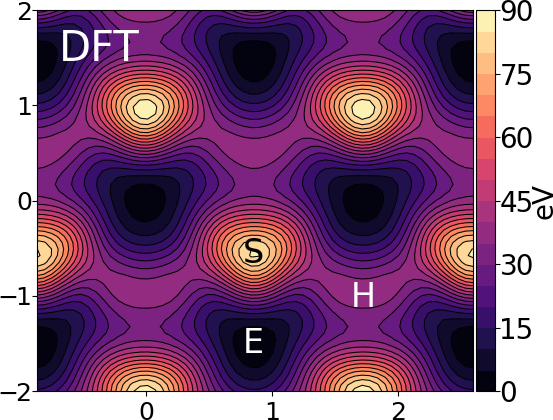
\includegraphics[width=0.5\textwidth]{Images/peierls_potential_dft_labelled_zeal.png} \\
             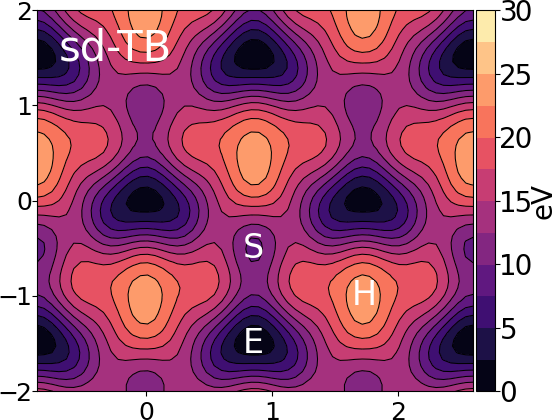
\includegraphics[width=0.5\textwidth]{Images/peierls_potential_sdTB_labelled_zeal.png}  \\
             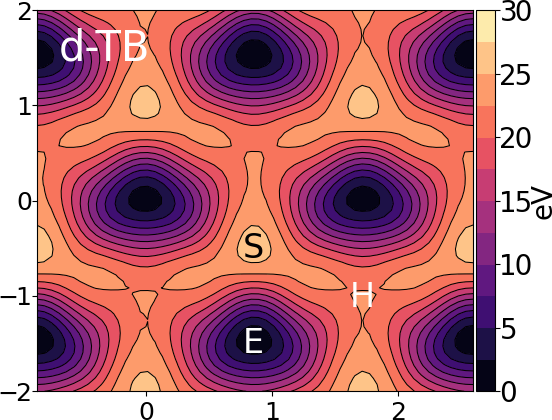
\includegraphics[width=0.5\textwidth]{Images/peierls_potential_dTB_labelled_zeal.png}  \\
    \end{tabular}
\caption{Comparison of 2d Peierls potentials of the $1/2\langle 111\rangle$ screw dislocation between DFT \cite{Itakura2012} (top) and tight-binding ($sd$ non-orthogonal middle, canonical d, bottom). $x-y$ axes in units of $d=a\sqrt{2} / 3$.Energy scale is in meV. "E", "H" and "S" correspond to easy, hard and split core positions respectively, with the latter also corresponding to atomic positions. The relative energies between the different core positions is smaller in tight-binding compared to DFT. The split core as seen in tight-binding is reminiscent of EAM potentials, where the split core energy is lower than that of the hard core. The discrepancy is probably due to an insufficient repulsion at close range within the tight-binding model.}
	\label{fig:peierlspot}
    \end{figure}



Comparison of 2d Peierls potentials of the \(1/2\langle 111 \rangle\)
screw dislocation between DFT and tight-binding models can be found in
figure \ref{fig:peierlspot}, with data found in table
\ref{tab:peierlspot}. The sampled energies were interpolated using 2d
cubic splines. The relative energies between the different core
positions was found to be smaller in both tight-binding models compared
to DFT. These are artifacts of the models, which have been reproduced in
atomistic NEB calculations of the \(1/2\langle 111\rangle\) screw
dislocation Peierls barrier using the canonical \(d\text{-band}\) model:
the Peierls barrier in this model is approximately half
that of DFT \cite{Simpson2019}.

The Peierls potential of the \(d\text{-band}\) model was found to be more
reminiscent of DFT, compared to the \(s\text{-d}\) model; but the
deviation is small: the maximum difference between the \$d\$/\(s\text{-}d\)
models being \(\sim 10\) meV, with the \(d\text{-band}\) model being, on average,
\(\sim+3\) meV higher.

The split core energy is lower than that of the hard
core, which is reminiscent of EAM potentials \cite{Itakura2012}, but not
as severe, as seen in figure \ref{hardsplittransition}. Some of
this discrepancy can be attributed to the to erroneous interaction term
included by Itakura, as detailed above---interaction energies can become
arbitrarily high, if not made independent of truncation limit---but
likely there are effects in DFT which are not encapsulated fully within
the tight-binding description, such as a lack of core electron repulsion
upon deformation of the lattice, which would increase the relative
energy difference. Consequences of this discrepancy on future kMC
simulations are discussed in section \ref{sec:discussion}.


\begin{table}[htbp]
\caption{Table of energies used to calculate the Peierls potential. All values in meV. \(\Delta E_{\text{P}}^{\text{DFT}}\) values taken from \cite{Itakura2012}. \label{tab:peierlspot}}
\centering
\begin{tabular}{rrrrrr}
Pos & \(\Delta E_{\text{INT}}\) & \(\Delta E_{\text{tbe}}\) & \(\Delta E_{\text{P}}^{sd}\) & \(\Delta E_{\text{P}}^{d}\) & \(\Delta E_{\text{P}}^{\text{DFT}}\)\\
\hline
1 & 0 & 0 & 0 & 0.0 & 0\\
2 & -0.7 & 7.3 & 7.9 & 6.3 & 3.2\\
3 & -1.4 & 16.0 & 17.4 & 15.1 & 19.2\\
4 & -2.0 & 22.2 & 24.2 & 20.4 & 31.1\\
5 & -2.5 & 24.8 & 27.4 & 22.6 & 39.3\\
6 & -3.3 & 3.0 & 6.3 & 4.6 & 11.5\\
7 & -6.5 & 7.1 & 13.6 & 12.7 & 39.9\\
8 & -9.6 & 13.0 & 22.6 & 22.7 & 75.2\\
9 & -12.5 & 5.4 & 17.9 & 26.8 & 108.9\\
10 & -4.8 & 22.1 & 26.9 & 23.0 & 34.8\\
11 & -7.2 & 18.2 & 25.4 & 23.5 & 37.9\\
12 & -9.8 & 14.0 & 23.8 & 24.4 & 60.7\\
13 & -3.8 & 11.5 & 15.3 & 13.2 & 17.6\\
14 & -6.9 & 15.1 & 22.0 & 20.3 & 29.9\\
15 & -4.3 & 18.6 & 22.9 & 20.0 & 39.7\\
\end{tabular}
\end{table}




        \begin{figure}
\centering
    \begin{tabular}{cc}
	     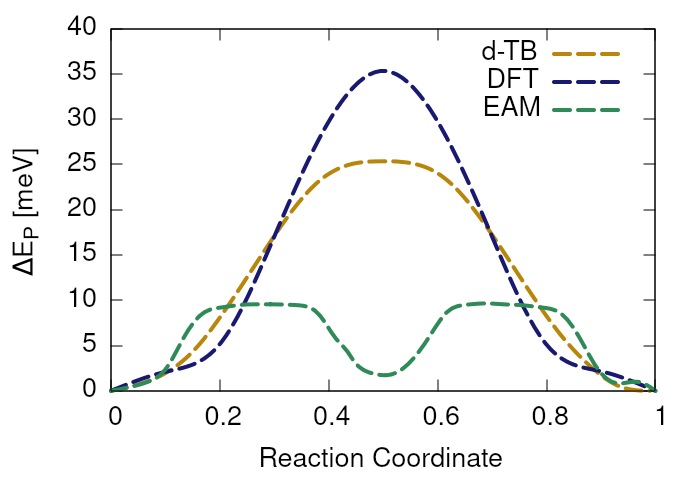
\includegraphics[width=0.5\textwidth]{Images/peierls_potential_atomistic_results.png} &
             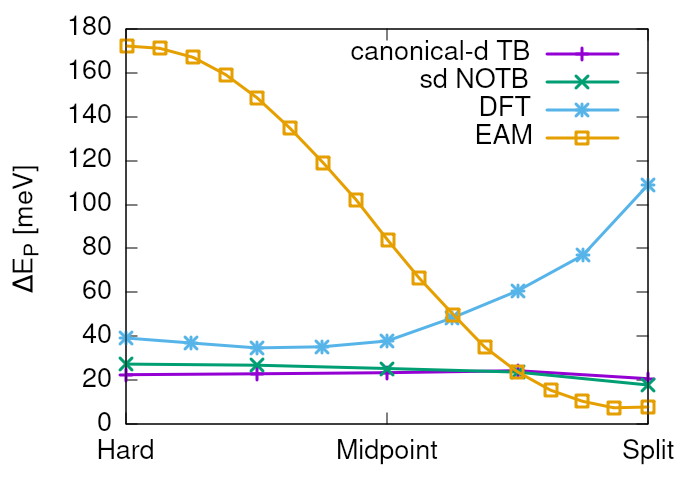
\includegraphics[width=0.48\textwidth]{Images/hard-split_transition_w_canonical.png}  \\
a) & b)\\
    \end{tabular}
\caption{Left: Peierls potentials produced from $d\text{-band}$ tight-binding, DFT and EAM along each of their respective the minimum energy pathways (right), which are the reaction coordinates for the figure on the right. The EAM potential of Mendelev \cite{Mendelev2003} has an unphysical well in the centre of the potential, while tight-binding and DFT produce single-humped potentials. Right: Peierls potential along the hard-split line. One can see in $s\text{-}d$ tight-binding model pathway is similar in shape to the EAM potential of Mendelev \cite{Mendelev2003}: it decreases consistently from the hard core to the split core. In DFT one finds a saddle point between the hard core and the midpoint. }
   \label{hardsplittransition}
    \end{figure}


The transitional kink shape from the \(s\text{-}d\) and \(d\text{-band}\) Peierls
potentials may differ compared to DFT, with dislocation core positions
possibly being situated closer to the split core position, similar to EAM
potentials \cite{Itakura2012,Mendelev2003}. Following the Peierls potential
along the H-S direction, as seen in figure \ref{hardsplittransition}, we see
that the Itakura potential has a saddle point minimum, which corresponds to
the dislocation core positions found upon kink-pair formation
\cite{Itakura2012}. In the \(s\text{-}d\) model, the Peierls potential decreases
monotonically along the H-S line and there is a subtle maximum found in the
\(d-\text{band}\) model. This data suggests there may be a deviation in the
dislocation path found in DFT, in moving from one peierls valley to the next along the H-S line. Atomistic calculation of
the Peierls barrier between two easy core positions in the canonical
\(d\text{-band}\) model found core positions of the transitional kink state to
go through the metastable point, similar to DFT \cite{Simpson2019}, which
suggest the deviation may not be severe. Section \ref{sec:ltmodel} discusses the
effect the Peierls potential has on the pathway taken by a
dislocation moving from one Peierls valley to the next.

\subsection{Preliminary calculations}
\label{sec:orgf7b4743}


To validate the cluster simulation method, the excess energy, defined as the difference in energy
between a cell with a dislocation, and a perfect reference cell, was plotted as as function of
\(\text{ln}(R/r_c)\), where \(R = R_2\) of the cluster and \(r_c = b\), as seen in
figure \ref{lnrdep}. In isotropic elasticity theory, this should give a linear dependence where the gradient
corresponds to \(\mu b^2 / 4\pi\), with the \(y\) intercept corresponding to the
core energy \(E_{\text{core}}\). This is well reproduced by our model, except at low \(\text{ln}(R/r_c)\)
as expected, where the cell size is not large enough to accommodate for sufficient relaxation of
the dislocation core, increasing the core energy, which is not accounted for in elasticity theory.


\begin{figure}[htbp]
\centering
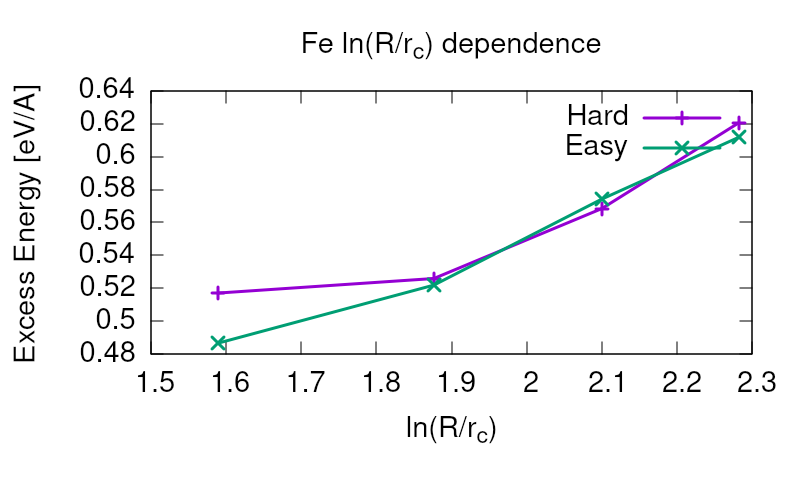
\includegraphics[width=0.7\textwidth]{/home/tigany/Documents/docs/Management/Images/img_fe_size_dependence_on_log_of_core_radius.png}
\caption{Excess energy of dislocation clusters with differing radii for both the easy and hard core configurations. The prediction from elasticity theory is given by the black, dashed line. Deviation of both cores occur when cell size is small, creating an increase in the core energy, which elasticity theory cannot account for. \label{lnrdep}}
\end{figure}




The energy cost to transform from the easy to the hard core can be estimated by
the difference in excess energies between the cores in the limit of
\(\text{ln}(\frac{R}{R_0}) \rightarrow 0\). At the smallest measured value, one finds that the core energy
difference \(\Delta E_{\text{core}}^{\text{Easy-Hard}} = 76\) meV/b, which is in good agreement with the DFT
value of 82 meV/b \cite{Itakura2012}.


For a line tension model of a dislocation, it is necessary to
ascertain the energy, denoted \(E_{\text{L}} = E_{\text{el}} + E_{\text{core}}\) as in Proville
\cite{Rodney2009}. This can be obtained by subtracting the total
energies of relaxed dislocation configurations to obtain the core
energy. 



\subsection{Fe-C binding energies}
\label{sec:org68d00d4}
\label{sec:fec_binding}

As found in DFT simulations by Ventelon \cite{Ventelon2015}, when a carbon was placed in the
vicinity of a relaxed easy dislocation core---in either of the two nearest, distinguishable,
octahedral sites---a spontaneous reconstruction of the dislocation core occurred: from easy to
hard. Upon reconstruction, the dislocation core moved to a neighbouring triangle, when looking
along the \(\langle 111\rangle\) direction, where the carbon found itself situated in the centre. This will be
called a prismatic site, as in Ventelon's paper. This confirms that both hard and easy
dislocation cores must be studied to fully understand screw dislocation behaviour in bcc iron.


The binding energies of carbon to both the hard and easy cores can be seen in table
\ref{tab:bindingenergies}, with the resulting distribution of carbon in figures
\ref{easybindingenergydist} and \ref{hardbindingenergydist}. The distribution of carbon strongly
depends on the type of core it finds itself situated near. The easy core only significantly
modifies the position of the iE1 site, to the E1 site, situated in the centre of an adjacent
triangle. All other sites are unaffected, so there is a one-to-one correspondence between all
\(\text{iE}j\) and \(\text{E}j\) sites, where \(j \in \{2\dots10\}\). There are carbon basins available close
to the triangular region containing the core, but not inside.

Carbon favours a prismatic site within the hard core (H1), which has the highest
binding energy, 1.29 eV, of all sites considered. There are no binding sites apparent in a triangular
annulus (of width \(a_{\text{bcc}}\sqrt{2}/2\)) surrounding the hard core triangle due to the
destruction/volume reduction of octahedral sites near the hard core. The initial octahedral
sites, iH1 and iH2 decay to the H1 site. Similarly, iH3 and iH4 decay to the H2 site, with iH9
and iH10 decaying to a H7 site. Relations between each of the sites is given in table
\ref{decayrelations}.


\begin{table}[htbp]
\caption{Decay relations between the initial and final sites upon relaxation of carbon intersitials around the hard core. \label{decayrelations}}
\centering
\begin{tabular}{ll}
Initial & Final\\
\hline
iH1, iH2 & H1\\
iH3, iH4 & H2\\
iH5 & H3\\
iH6 & H4\\
iH7 & H5\\
iH8 & H6\\
iH9, iH10 & H7\\
\end{tabular}
\end{table}


Note that interactions between carbon atoms around the core are not taken into account here:
figures \ref{easybindingenergydist} and \ref{hardbindingenergydist} are purely diagrammatic and not
what one expects the true distribution of carbon around a screw dislocation would be. Carbon is strongly
repulsive at first nearest-neighbour distances, which would modify each of these
distributions. 


 \begin{figure}
\centering
     \begin{tabular}{l}
 	           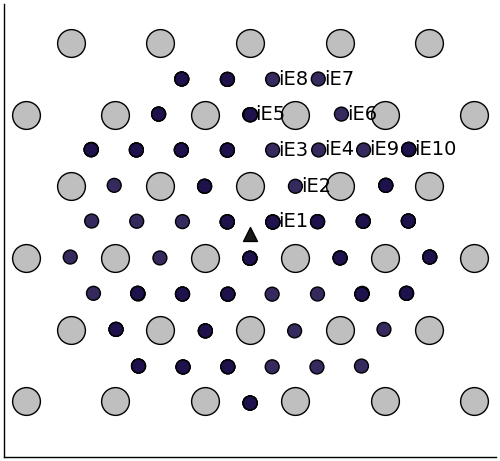
\includegraphics[width=0.7\textwidth]{Images/easy_core_fe_C_initial_positioning.png}  \\
 	           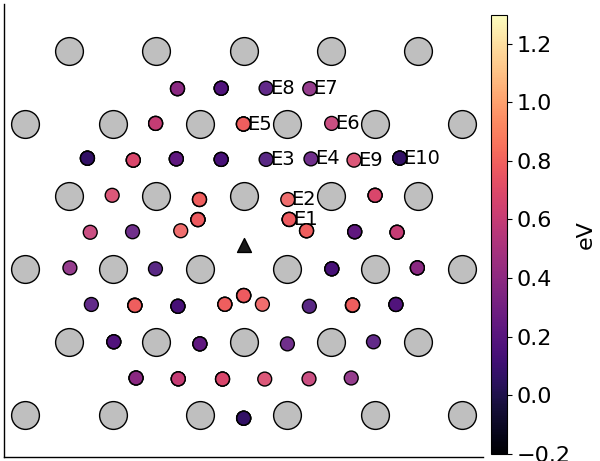
\includegraphics[width=0.85\textwidth]{Images/easy_core_fe_C_positioning_energies_e10_label.png}  \\
		   
     	      \end{tabular}		
 \caption{ Initial (top) and final (bottom) positions and binding energies (eV) of carbon around the easy core. Binding energies are not shown for the initial positions. Top: initial positions before relaxation. Bottom: final positions and binding energies after relaxation. The core was constrained by fixing the top and bottom three atoms surrounding each of the cores. As shown by Ventelon \cite{Ventelon2015}, the first and second closest octahedral sites to the hard core decay to a prismatic position inside the hard core. }
 \label{easybindingenergydist}
    \end{figure}


 \begin{figure}
\centering
     \begin{tabular}{l}
 	           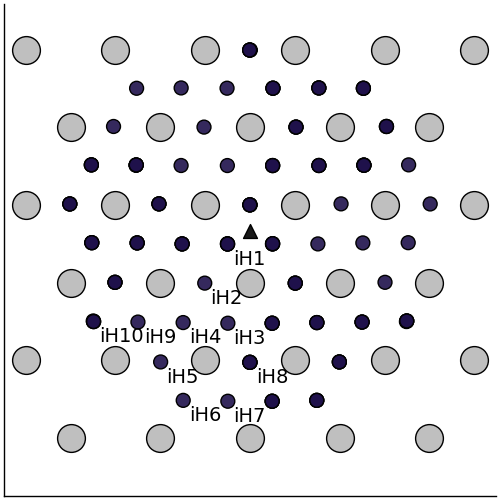
\includegraphics[width=0.7\textwidth]{Images/hard_core_fe_C_initial_positioning.png}  \\
 	           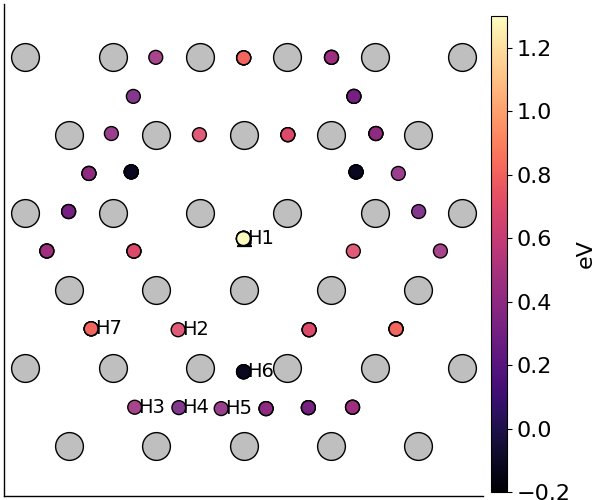
\includegraphics[width=0.85\textwidth]{Images/hard_core_fe_C_positioning_energies_h7_label.png}  \\
		   
     	      \end{tabular}		
 \caption{ Initial (top) and final (bottom) positions and binding energies (eV) of carbon around the hard core. The core was constrained by fixing the three atoms surrounding each of the cores in the top and bottom layers. As shown by Ventelon \cite{Ventelon2015}, the first and second closest octahedral sites to the hard core decay to a prismatic position inside the hard core. }
 \label{hardbindingenergydist}
    \end{figure}




    \begin{table*}
\centering
	\begin{tabular}{cccccc}
	\hline
    Site Type & distance from core [b] & $E^{z}$ [eV] & $\Delta E^{z}$ [eV] & $E_b$ [eV] & $E_b^{z}$ [eV]  \\ 
    	 \hline
    % 00        &                    --  &   0.203      &               0.000 &             &         --     \\
    %           &                        &              &                     &             &                \\\hline
    E1        &                   0.57 &   0.185      & 	     -0.018 &       0.793 &          0.775 \\
    E2        &                   0.70 &   0.202      & 	     -0.001 &       0.793 &          0.793 \\
    E3        &                   0.99 &   0.205      & 	      0.002 &       0.137 &          0.139 \\
    E4        &                   1.21 &   0.208      & 	      0.005 &       0.229 &          0.234 \\
    E5        &                   1.36 &   0.210      & 	      0.008 &       0.784 &          0.791 \\
    E6        &                   1.66 &   0.209      & 	      0.007 &       0.597 &          0.603 \\
    E7        &                   1.89 &   0.206      & 	      0.003 &       0.385 &          0.388 \\
    E8        &                   1.77 &   0.203      & 	      0.000 &       0.177 &          0.178 \\
    E9        &                   1.52 &   0.201      & 	      0.000 &       0.683 &          0.683 \\
    E10       &                   1.95 &   0.202      & 	      0.000 &       0.067 &          0.067 \\ \hline
    H1        &                   0.00 &   0.196      & 	     -0.006 &       1.298 &          1.291 [ 0.881\textsuperscript{a}, 0.790\textsuperscript{b}  ] \\
    H2        &                   1.19 &   0.210      & 	      0.007 &       0.691 &          0.698 \\
    H3        &                   2.12 &   0.209      & 	      0.007 &       0.461 &          0.467 \\
    H4        &                   1.91 &   0.207      & 	      0.005 &       0.311 &          0.316 \\
    H5        &                   1.80 &   0.208      & 	      0.006 &       0.403 &          0.409 \\
    H6        &                   1.40 &   0.207      & 	      0.005 &      -0.119 &         -0.114 \\
    H7        &                   1.35 &   0.206      & 	      0.006 &       0.825 &          0.819 \\
    
	\end{tabular}		
 	\caption{Table of energies leading to the zero-point energy corrected binding energy using the cluster method for simulation of dislocation-carbon interactions. \textsuperscript{a} Tight-binding quadrupolar array results, starting from a fully relaxed easy core quadrupole extended to a depth of 3b with carbon introduced into the iH1 site in the middle layer, by both dislocations. \textsuperscript{b} DFT results of Ventelon, using the same quadrupolar configuration as in \textsuperscript{a}. In both quadrupolar simulations, carbon ended up in the H1 site.}
	\label{tab:bindingenergies}
    \end{table*}

These binding energies agree well with experiment and atomistic/elastic calculations. EAM simulations
by Clouet \cite{Clouet2008,Becquart2007} found a maximum binding energy of 0.41 eV by calculating
the elastic dipole tensor within Eshelby theory. Hanlumyuang et al. \cite{Hanlumyuang2010},
similarly conducted DFT and EAM calculations for the interaction energy 12\AA{} from the core, and
their calculations agreed with the continuum limit of Eshelby theory with a binding energy of
0.2 eV. In DFT calculations by Ventelon \cite{Ventelon2015}, the interaction energy of a carbon in a
hard core prism configuration was found to be 0.79 eV for a thickness in the \(Z\) direction of
3\(b\) (0.73eV for \(6b\))---in the convention that a positive binding energy indicates
attraction. This is significantly lower than the 1.29eV interaction energy of tight-binding.
This discrepancy can be partially explained by the fact that the cells have not been allowed to
relax with all degrees of freedom, as in the Ventelon results: the three atoms around the screw
core are fixed in \(Z\) to so the dislocation core position does not change upon
relaxation. 

Repeating the calculation for the binding of a H1 carbon to a screw
dislocation using a quadrupolar array, allowing for all atoms to relax, gives a
binding energy of 0.88 eV. This agrees very well with the DFT results of Ventelon
\cite{Ventelon2015}.

A source of error for this discrepancy is likely from the fitting of the tight-binding model
itself. The Peierls barrier of this \(s\text{-}d\) model of iron, necessary for Fe-C
interactions, has been shown to be half that found in DFT \cite{Simpson2019}, but the
solution energies for Fe-C defect complexes are well described. This implies there is
insufficient repulsion between Fe-Fe species upon deformation, leading to a larger
resultant Fe-C binding energy from tight-binding.



\subsection{Carbon concentration along on line}
\label{sec:orgbe30f4c}

The variation of carbon concentration along the dislocation line for the highest
binding energy sites of the easy and hard cores can be seen in figure
\ref{cdhardeasy}. We see at low temperatures, all dislocations are
decorated with carbon. As temperature increases, the amount of carbon
decorating the dislocations starts to decrease. Due to the lower binding
energy of carbon to the easy core, desaturation occurred at a lower
temperature compared to the hard core. Dislocation densities near the upper
bound of what has been observed in martensite, \(\rho \approx10^{15}\), reduce
the temperature at which carbon concentration starts to decrease on the
dislocation core. Lower nominal carbon concentrations cause carbon
concentrations around the dislocation to decrease at a lower temperature.

In the high-purity iron case, \(C_{\text{nom}} = 10\) appm, we find at
dislocation densities above \(\rho \approx10^{15}\), that there is a reduction
in the maximum concentration permitted in the material, with increasing
dislocation density. This is due to the fact that there is not enough carbon
for all of the dislocations, as such the concentration on the dislocation line
drops.

In the operating temperature range of \(40-90\deg\text{C} = 310-360\deg\text{K}\), we expect most hard
core sites are saturated. Given the high concentrations of the E1/E2 sites around the easy core
in this range, we expect all dislocations will be of the hard core type, due to reconstruction of
the easy core by the adjacent carbon.

\begin{landscape}
 \begin{figure}
  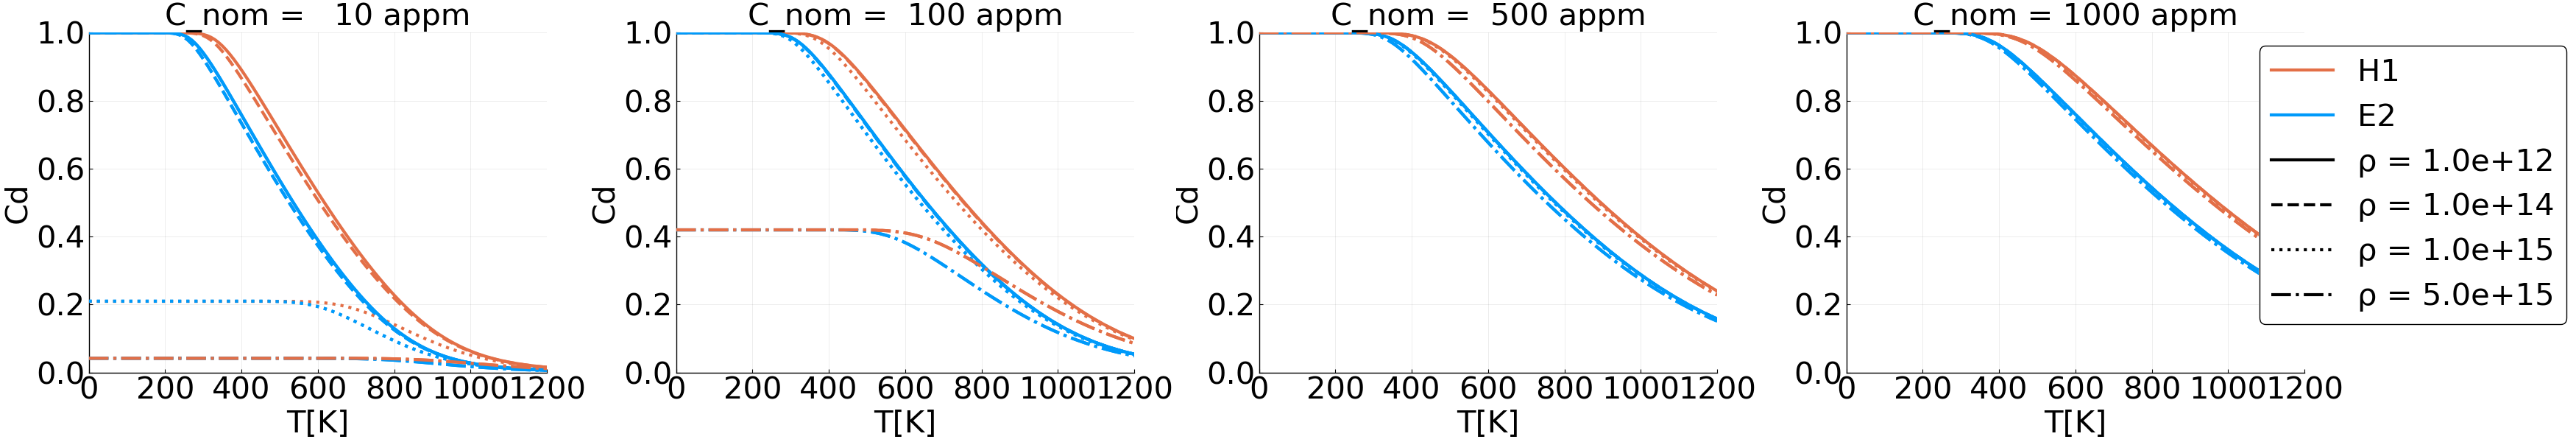
\includegraphics[width=1.6\textwidth]{Images/mcclean_isotherm_all_e2_h1.png}
   \caption{Variation of carbon concentration on the dislocation line $c_d$ for the highest-energy binding sites for the hard core (H1) and easy core (E2). Solid, dashed, dotted and dash-dotted lines correspond to dislocation densities of $1\times10^{12}$, $1\times10^{14}$, $1\times10^{15}$ and $5\times10^{15}$ respectively. The nominal carbon concentrations are 10, 100, 500 and 1000 appm from left to right, where around 1000 appm corresponds to the concentration of carbon at the solubility limit of C in ferrite: 0.02wt\%. $c_d$ and $c_{\text{bulk}}$ reached self-consistency, with an absolute tolerance of $1\times 10^{-6}$. C-C interactions were taken into account with the repulsive first-neighbour interaction energy $V_{\text{CC}}=0.21$ eV. No intersite interactions were taken into account. The maximum concentration of carbon around the easy core, drops off at a lower temperature than that of the hard core due to lower binding energy of the E$2$ site compared to the H1 site. The operating temperature is taken to be $50\deg$ C $= 320 \deg$ K.}\label{cdhardeasy}
\end{figure}
\end{landscape}



The C-C first-neighbour repulsive energy present of carbon in a
site was found for the H1 site using a quadrupolar configuration.
It was found to be 0.75 eV, which is quite off DFT, now just
recalculating using different reference cells for the carbon
configurations.





\subsection{Line Tension Model}
\label{sec:org54471c0}
\label{sec:ltmodel}
\subsubsection{Prerequisites}
\label{sec:orgd708cba}

The \(K\) coefficient for the line tension model was calculated from atomistic simulations, using
the method of Itakura \cite{Itakura2012}, by calculation of a Hessian from the displacement of
atoms surrounding the dislocation core. Tight-binding gave \(K = 0.734\) eV\AA{}\(^{-2}\), which agrees well
with DFT, where \(K = 0.816\) eV\AA{}\(^{-2}\).


[\begin{figure}[htbp]
\centering
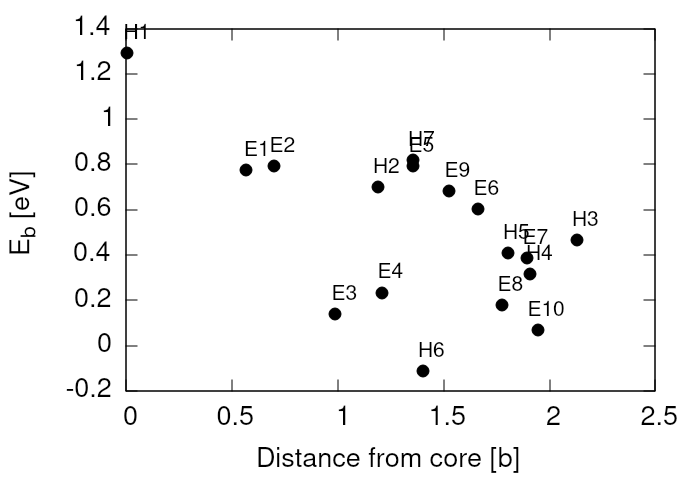
\includegraphics[width=0.7\textwidth]{/home/tigany/Documents/docs/Management/Images/fe_c_binding_energy_distance.png}
\caption{Distance dependence of the binding energies of carbon to the \(1/2\langle 111 \rangle\) screw dislocation in iron. Positive binding energies denote a favourable binding. \label{distancedep}}
\end{figure}]

Dislocation-carbon binding energies were found to decay with distance, as seen in figures
\ref{distancedep} and \ref{lorentzianfit}. A Lorentzian was fit to specific binding energies such
that a continuous function could be used to describe binding within
the line tension model. This is a purely empirical model. The
choice of sites used for the fitting is discussed in section
\ref{sec:discussion}.

This distance-dependence agrees well with previous
calculations of the binding energy at larger distances from the core
\cite{Hanlumyuang2010}.

\textbf{ELASTIC DIPOLE CALCULATION?}




\begin{figure}[htbp]
\centering
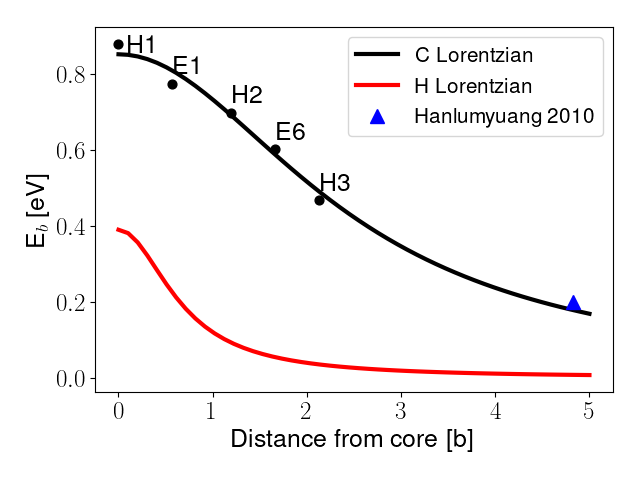
\includegraphics[width=0.7\textwidth]{Images/binding_energy_dependence_C_H_lorentzian_with_scatter.png}
\caption{Parameterised distance dependence of carbon binding energies to the \(1/2\langle 111 \rangle\) screw dislocation in iron. The sites chosen to fit to were determined by those sites a prismatic carbon in a hard core configuration would find itself, if the dislocation were to move without it along the \(X = \langle\bar{2}11\rangle\) direction. The triangle, labelled Hanlumyuang, refers to the binding energy resulting from measurement of the elastic dipole tensor from DFT calculations evaluated at \(12\AA\) \cite{Hanlumyuang2010}. Binding energy of hydrogen to the \(1/2\langle 111 \rangle\) screw dislocation also shown for comparison \cite{itakura13_effec_hydrog_atoms_screw_disloc} \label{lorentzianfit}}
\end{figure}

\subsubsection{Kink-pair formation in pure iron}
\label{sec:org14c30fe}

The kink-pair formation enthalpy is defined as the minimum energy necessary
to to create a kink-pair from a dislocation in a Peierls valley. One
can find this by sampling the energy landscape seen by a dislocation line
which moves one peierls valley to the next, from which the minimum enthalpy
path can be sought. The difference of the energy maxima of a dislocation state along the minimum
enthalpy path (MEP) relative to the
initial state, is the kink-pair formation energy. One can efficiently
determine the minimum enthalpy path using the String/Nudged Elastic Band
(NEB) algorithms. In these methods, a set of images, which interpolate
between the initial and final states, are relaxed along the energy
landscape.

A \texttt{julia} implementation of the string algorithm, accelerated by use
of an ODE solver, was used to relax the images \cite{Makri2019}. The
implementation was validated on the dataset of Itakura \cite{Itakura2012}.

\begin{figure}[htbp]
\centering
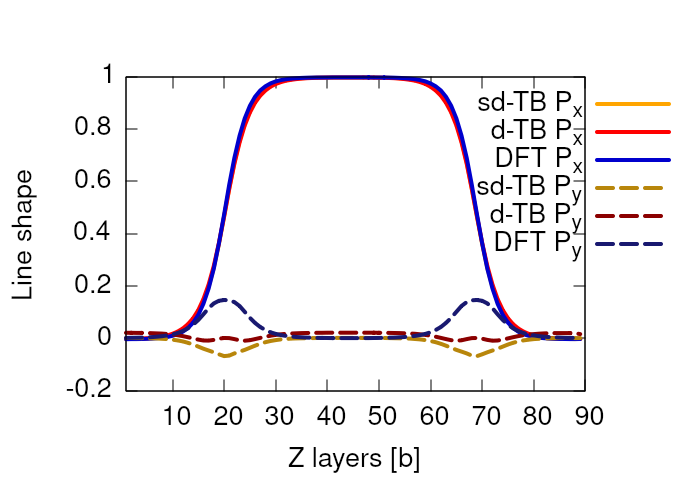
\includegraphics[width=0.7\textwidth]{Images/lineshape-all_correct_gradient.png}
\caption{Core positions of the line tension model from DFT (blue) and tight-binding (yellow) for the middle image corresponding the MEP and the kink-pair formation energy. Images were relaxed using the ODE String method of Makri and Ortner \cite{Makri2019}. \(P_x\) and \(P_y\) correspond to the x/y-coordinate of the dislocation core position in each of the discretised layers of the dislocation. One finds that the kink width in tight-binding is wider than that found in DFT, which corresponds with the fact that the width is proportional to \(b\sqrt{K/\Delta E_P}\), where the reduction in \(\Delta E_P^{\text{tbe}}\) is greater than the reduction in \(K_{\text{tbe}}\).   \label{lineshape}.}
\end{figure}



In figure \ref{lineshape}, one can see the \(P_x\) and \(P_y\) core positions which
result from the highest enthalpy image of kink-pair formation for the
canonical-\(d\) and \(sd\) tight-binding models, where the DFT comparison is from
\cite{Itakura2012}. Plots of the corresponding dislocation core pathway, \(P_j =
    (P^j_x, P^j_y)\), looking down the dislocation line, are shown in
\ref{easyeasytransition}.

The \(P_x\) line shape agrees well with the DFT-based results. The kink width
was found to be slightly wider: \(11b\) in tight-binding from the line-tension
model, compared to \(10b\), in DFT \(10b\). This results from the fact that the
width is proportional to \(b\sqrt{K/\Delta E_P}\), where the reduction in
\(\Delta E_P^{\text{tbe}}\) is greater than the reduction in \(K^{\text{tbe}}\)
\cite{Itakura2012}. Differences in the \(P_y\) line shape are noticeable, with
the canonical-\(d\) model reproducing the result closest to the DFT \(P_y\) line
shape.


The differences in these line shapes manifest themselves clearly in
plots of the dislocation pathway, figure \ref{easyeasytransition}, where
the core migration path dips below the midline in both the
\(d\) and \(sd\) models, with a more pronounced effect being shown by the \(sd\)
model. Apart from this discrepancy, we see there is good agreement between
tight-binding to DFT when compared to the EAM potential of Mendelev
\cite{Mendelev2003} in which we see a path which passes close to the split-core
position. This is expected due to the low value of the Peierls potential of
the EAM, as seen in figure \ref{hardsplittransition}.



\begin{figure}[htbp]
\centering
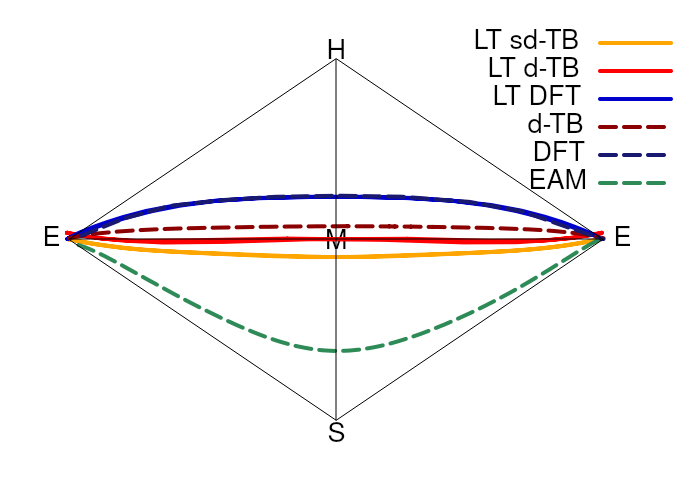
\includegraphics[width=0.7\textwidth]{Images/easy-easy_transition_pathway_combined_dTB_sdTB_DFT_EAM_dotted_smooth_colour.png}
\caption{Comparison of minimum energy pathways from different atomistic calculations to the line-tension model. Dashed lines correspond to atomistic calculations. Solid lines are results from the line-tension models. Tight-binding follows a pathway much closer to that of DFT. EAM potentials predict that the dislocation core goes to the split core and then back to the easy core. Even though the Peierls landscape found in tight binding has similar characteristics to the EAM in terms of the energetic ordering of different core states, the description of the minimum energy pathway of the \(1/2\langle 111 \rangle\) screw dislocation as it moves between core positions is in good agreement with DFT. \label{easyeasytransition}}
\end{figure}



In the EAM model, the midpoint along the hard-split transition is not a saddle
point. The MEP for kink-pair formation deviates widely from the DFT path.



The kink-pair formation enthalpies obtained from the tight-binding models can
be found in table \ref{kink-pair_formation_enthalpy_pure}. Tight-binding
underestimates the kink-pair formation enthalpy by \(0.18\) eV, in comparison to
DFT. This can largely be attributed to the difference in Peierls potentials
between DFT and tight-binding.

\begin{table}[htbp]
\caption{Kink-pair formation energies between DFT, and the two flavours of tight-binding used with the line-tension model \label{kink-pair_formation_enthalpy_pure}.}
\centering
\begin{tabular}{ll}
Method & \(E_{\text{kp}}^{\text{form}}\)\\
\hline
DFT & 0.71 eV\\
TB (sd-non-orthog.) & 0.56 eV\\
TB (d-orthog.) & 0.53 eV\\
\end{tabular}
\end{table}


\subsubsection{Kink-pair formation enthalpy with a single carbon}
\label{sec:orge108a11}

To understand how kink-pair nucleation is affected by carbon, one
can study the formation of a kink-pair of a dislocation going from one
peierls valley to the next---as in the previous section---but with the
additional interaction of a single carbon atom with the
dislocation.

We place carbon in the E1 site, the highest binding energy site of carbon to
the easy dislocation core. The carbon is fixed in place during kink-pair
formation, as such we are assuming a regime in which the dislocation
velocity is much greater than the diffusion of carbon. Carbon-dislocations
interactions are only permitted between the dislocation segment closest to
the carbon.


    \begin{figure}
\centering
	\begin{tabular}{r}
		      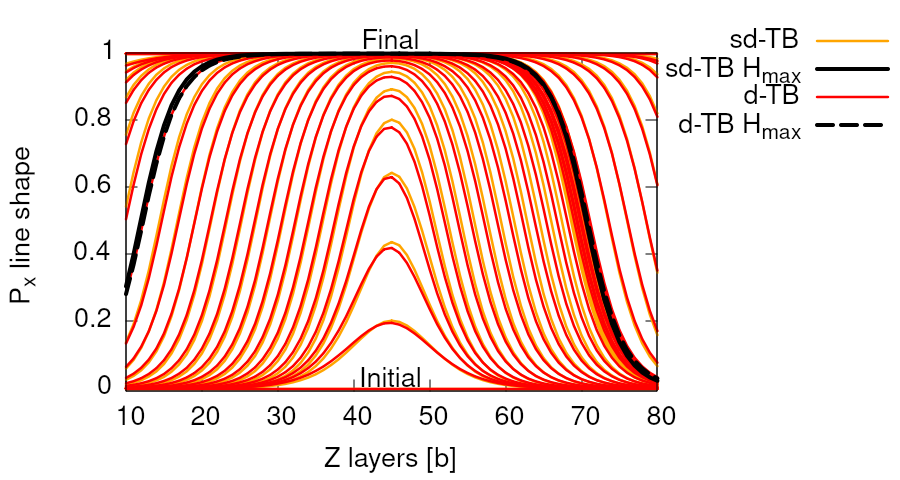
\includegraphics[width=0.75\textwidth]{Images/lineshape_no_carbon_sd_dTB_off_kilter_hmax_label.png} \\
		      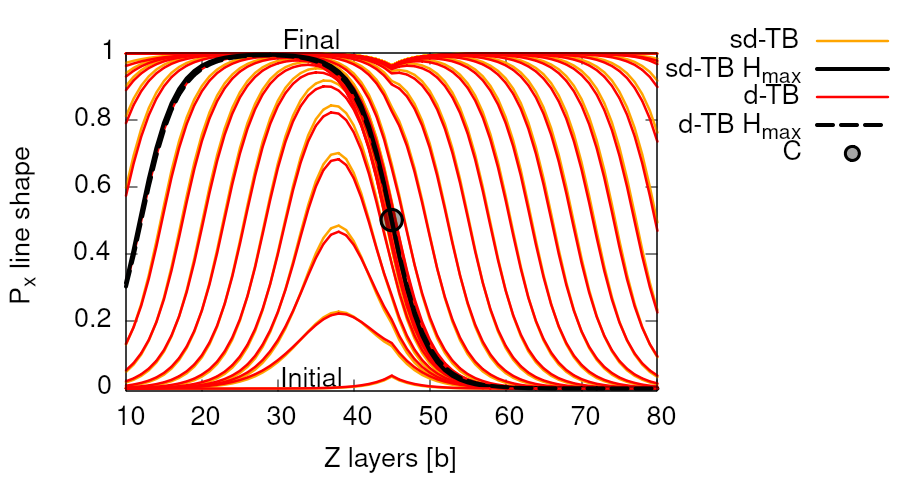
\includegraphics[width=0.75\textwidth]{Images/lineshape_with_carbon_sd_dTB_off_kilter_hmax_label.png}  \\

		 \end{tabular}
    \caption{ Comparison of $P_x$ lineshapes for the $sd$ and $d$ models in pure iron (top) and iron with a single carbon interacting with the central dislocation segment in E1 site (bottom). The highest enthalpy images, $H_{\text{max}}$, for each of the models are shown in black. In pure iron, the $d$ model lineshapes are offset from the $sd$ due to the different Peierls potentials involved. With carbon along the path of migration, we find the dislocation intersects the solute, due to its large binding energy.}
    \label{fig:alllineshapes}
       \end{figure}


\(P_x\) line shapes obtained during kink-pair formation can be seen in figure
\ref{fig:alllineshapes}. The addition of carbon causes a cusp in the
dislocation line towards the carbon in the initial and final images, due to
the reduction in potential the central dislocation segment experiences due
to carbon interaction. As the dislocation bows out to form a kink pair, the
cusp becomes less prominent. As we reach the transition state, the dislocation
image intersects the carbon position, to minimise energy.

The pathway corresponding to the highest enthalpy image, can be seen in
figure \ref{fig:pathwaysinglec}. Looking along a direction, we see the path a
dislocation takes in going between adjacent peierls valleys is asymmetric,
as expected due to the due to the strong binding of carbon.

These features agree very well with the line tension model in Itakura
\cite{itakura13_effec_hydrog_atoms_screw_disloc}, focussing on the case of
dislocations undergoing kink-pair formation in the presence of a single
hydrogen atom. Differences between the case of carbon and hydrogen
interaction will be discussed later.

\begin{figure}[htbp]
\centering
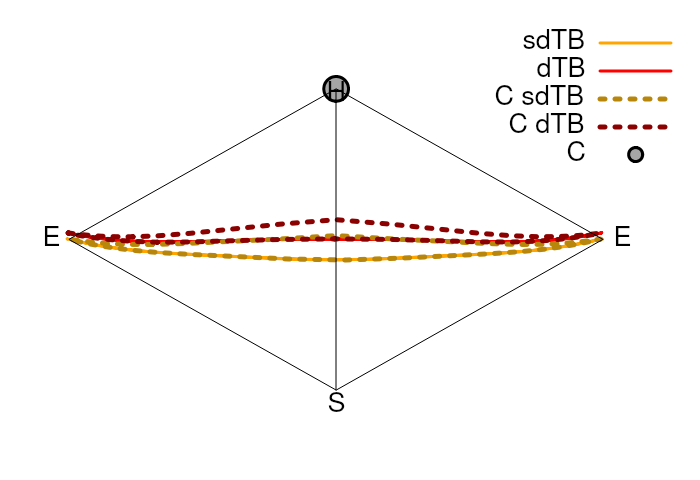
\includegraphics[width=0.8\textwidth]{Images/pathway_single_carbon_sd_d.png}
\caption{The migration path of the highest enthalpy images for both the \(sd\) and \(d\) tight-binding models with a single carbon in an E1 site. Carbon causes a deviation of the kink-pair formation path from the pure iron case (solid lines), due to carbon-dislocation binding. \label{fig:pathwaysinglec}}
\end{figure}


\begin{figure}[htbp]
\centering
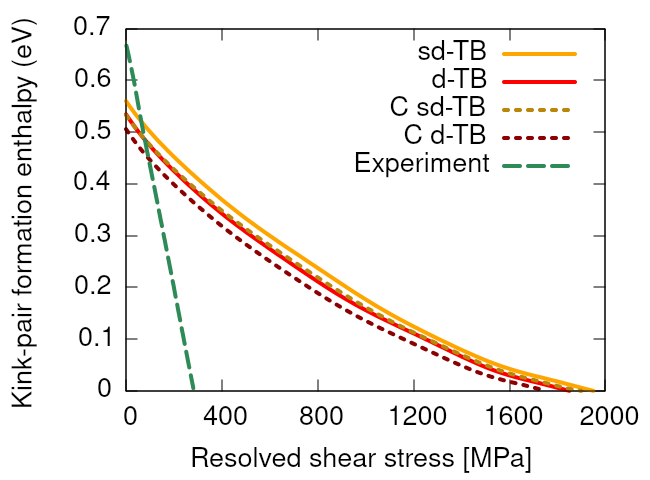
\includegraphics[width=0.8\textwidth]{Images/kink-pair_formation_enthalpies_dTB_sdTB_2000_big.png}
\caption{Dependence of the kink-pair formation enthalpy with increasing stress on the \([111](1\bar{1}0)\) direction. Solid lines: pure iron. Dotted lines: carbon ahead of the dislocation line in an octahedral site. Experimental data taken from Spitzig \cite{Spitzig_1970}. \label{kinkpairstress}}
\end{figure}



The kink-pair formation enthalpy of \(sd\) and \(d\) iron models, in both pure
iron, and with carbon ahead of the dislocation line are shown in figure
\ref{kinkpairstress}. The shape agrees well with results of the line tension
model of Itakura \cite{Itakura2012}, and from atomistic calculations of EAM
\cite{Proville2012} and GAP \cite{Maresca2018} potentials. We find that carbon
produces a consistent reduction of \(\sim 50meV\) to the kink-pair formation
enthalpy when placed ahead of the dislocation line. The reduction is
surprisingly small compared to the effect of hydrogen interaction with
dislocations \cite{itakura13_effec_hydrog_atoms_screw_disloc}, see figure
\ref{kinkpairstress}. The discrepancy between carbon and hydrogen is due to
the more gradual decrease of the carbon-dislocation interaction---over the
distance between the initial and transition states---compared to the
hydrogen-dislocation interaction. Comparing the two interaction functions,
we have at the peierls valley \(P_{\text{disl}}=(0,0)\), and \(P^{\text{H}} =
    P^{\text{C}} = (1.17\AA,0.68\AA)\) giving a distance \(d = 0.54b\) between the
dislocation and the solute. The difference in the interaction energy for a
dislocation segment in the final position in interaction for hydrogen
\(\Delta E_b^{\text{H}} = E_b(\text{H},0) - E_b(\text{H},0.54b) = 150 meV\),
whereas for carbon we have \(\Delta E_b^{\text{C}} = E_b(\text{C},0) -
    E_b(C,0.54b) = 40 meV\).



However, due to the longer range of the interaction function, we expect that
carbon will provide comparable decreases to the kink-pair formation up to
distances up to 5b, if placed ahead of the dislocation line.



The stress at which the kink-pair formation enthalpy becomes zero is the
Peierls stress. In the zero temperature limit, we can approximately account for quantum effects, such as
tunnelling and zero-point energy, by subtracting the Wigner correction,
determined by quantum transition state theory \cite{Proville2012,Henkelman2006}, from the
kink-pair formation enthalpy. Calculating this correction within tight-binding is currently
intractable. The correction has been calculated in the
Mendelev EAM potential \cite{Mendelev2003} for a screw dislocation undergoing
kink-pair nucleation \cite{Proville2012}. The Wigner correction obtained is
0.09eV. We find find that the Peierls stress obtained for both the \(sd\) and
\(d\) models is \$\(\approx\)1.2\$GPa, see table \ref{wignercorrection}.


\begin{table}[htbp]
\caption{Peierls stress of screw dislocation taken from the line tension model with the effect of the correction to the Peierls stress from quantum effects, estimated by Proville \cite{Proville2012}. The significantly lowers the enthalpy. Kink-pair formation enthalpy is reduced by roughly 50 MPa consistently due the the effect of carbon. \label{wignercorrection}}
\centering
\begin{tabular}{lrr}
Model & Peierls Stress [GPa] & Peierls Stress with Wigner correction [GPa]\\
\hline
sd-TB & 1.95 & 1.35\\
C sd-TB & 1.90 & 1.30\\
\hline
d-TB & 1.85 & 1.30\\
C sd-TB & 1.75 & 1.20\\
\end{tabular}
\end{table}







\begin{figure}[htbp]
\centering
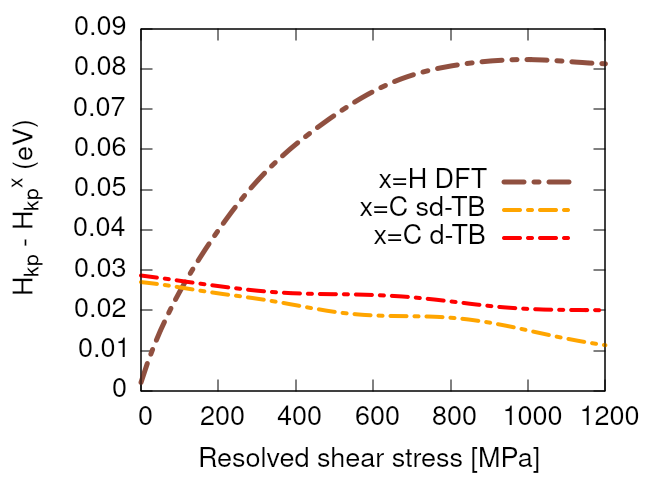
\includegraphics[width=0.8\textwidth]{Images/kink-pair_formation_enthalpy_difference_dft_comparison_big.png}
\caption{Difference in the kink-pair formation energy due to the addition of carbon. Comparison with hydrogen from work of Itakura \cite{itakura13_effec_hydrog_atoms_screw_disloc}.}
\end{figure}



Discrepancies in the kink-pair formation enthalpy compared to experimental
measurements of Spitzig \cite{Spitzig_1970}, can be attributed to multiple
sources. In bcc metals, experimental measurements of the CRSS, which can be linked to the
kink-pair formation enthalpy, are thought to measure the stress required to
operate Frank-Read sources which have been blocked due to the back stress of
generated screw dislocations \cite{Groger2007}. As mixed dislocations bow out
from the source, long screw segments form, due to the higher mobility of
mixed/edge character segments compared to screw segments. Between the source
and the screw dislocations, there are non-screw dislocations. The stresses
from these non-screw dislocations act in conjunction with applied stress, to
reduce the necessary CRSS by 2-3 times. As such the enthalpy barrier
obtained from the experimental CRSS measurements of Spitzig, cannot be
directly compared to the true kink-pair formation enthalpy necessary for a
single screw dislocation to undergo thermally-activated movement.

\subsubsection{Kink-pair nucleation rate}
\label{sec:orge537319}

As shown in Itakura \cite{itakura13_effec_hydrog_atoms_screw_disloc}, one can calculate the kink-pair nucleation rate using the Arrhenius law:

\[ R_N = \nu_d N_d \exp\big( \frac{- H_k(\sigma)}{k_{\text{B}}T} \big), \]

where \(\nu_d\) is the attempt frequency, \(N_d\) is the length of the dislocation
in burgers vectors, \(H_k(\sigma)\) is the kink-pair formation
enthalpy. Experimental results of \emph{in situ} straining of Fe from Caillard
\cite{Caillard2010}, enable calculation of the attempt frequency for stable
kink-pairs: assuming \(b = 2\mu\text{m}\), \(T=\) 300K and an applied stress of 33MPa
one obtains \(R_N = 81s^{-1}\).

There will be an enhancement of the rate due to carbon occupying sites ahead
of the dislocation. Given a concentration of carbon in the sites ahead
\(c_d \equiv c_d^{\text{E2}}\), the rate is enhanced by \(1 + c_d W_k \{ - \exp( \Delta
    H_{k}/k_{\text{B}}T ) - 1 \}\), where \(\Delta H_{k} = H_k - H_k^{\text{C}} =\)
30meV and \(W_k \sim 10b\) is the kink-width. Assuming
\(T=300\) K, this gives enhancement factors shown in table \ref{rateenhancement}.


\begin{table}[htbp]
\caption{Enhancement factors to the kink nucleation rate, where \(c_d\) was taken as the value reached from self-consistency at T=300K, at a dislocation density of \(\rho = 10^{15}\), as seen in figure \ref{cdhardeasy}. Kink-pair nucleation rate enhancements steadily increase until concentrations at which all dislocations are decorated with carbon, in the cases of \(C_{\text{nom}} \geq 500\). \label{rateenhancement}}
\centering
\begin{tabular}{rr}
\(c_{\text{nom}}\) [appm] & Nucleation Rate Enhancement factor\\
\hline
10 & 5.6\\
100 & 10.0\\
500 & 22.9\\
1000 & 22.9\\
\end{tabular}
\end{table}


These rate enhancements are an order of magnitude less compared to what one finds
with hydrogen in iron, due to the small difference to the kink-pair formation
enthalpy. However, this only accounts for a single carbon just ahead of the
core. Dislocations will have Cottrell atmospheres, as such, carbon at larger
distances ahead of the dislocatin core, up to 5b, will enhance the
nucleation rate by a similar amount.

For a significant enhancement, following the analysis of Itakura,
\(c_d\) must be similar in magnitude, or greater than

\[ c_d^E = \frac{1}{W_k \{\exp( \Delta H_{k}/k_{\text{B}}T ) - 1 \}}, \]


As temperature is raised, \(c_d^E\) increases, as \(c_d\)
decreases. Therefore, there exists a critical upper temperature, \(T_\text{U}\) where the
condition of \(c_d^E > c_d\) is not fulfilled. For the bulk concentrations of
carbon we have used, we find the upper critical temperatures to be

\begin{center}
\begin{tabular}{rl}
\(c_{\text{nom}}\) [appm] & \(T_\text{U}\) [K]\\
\hline
10 & \\
100 & \\
500 & \\
1000 & \\
\end{tabular}
\end{center}


The diffusion coefficient of carbon is \(D_0 = 1.67 \times10^-3\). Attempt
frequency is given by \(\nu_0 = 6D_0 / a^2\), which gives the attempt
frequency in the bulk to be \(\nu^{\text{C}}_b = 1.2 \times10^13 s^{-1}\) \cite{Jiang2003,daSilva1976}.




EAM calculations by Nematollahi \cite{Nematollahi2016}, find that the
migration energy barrier of carbon is significantly reduced around
dislocations, giving rise to a due to a "high mobility zone". They propose
screw dislocations drag carbon along during glide, and that pipe diffusion
of carbon on screw dislocations is unlikely. Measurement of the diffusion
barriers for carbon to move around a screw dislocation, there may be a
greater enhancement of the kink-pair nucleation rate, due to the diffusion
coefficient of carbon around dislocations being much higher than that of the
bulk. Tight-binding should provide a more accurate estimate of the migration
barrier than EAM calculations, due to its quantum mechanical description of
interatomic forces. Future work will be to measure this diffusion barrier to
determine if there are significant modifications to the kink-pair nucleation
rate.

\subsection{Line-tension equilibrium conditions}
\label{sec:org2ef5b4b}

\subsubsection{Dynamics of straight 1/2\(\langle 111 \rangle\) screw dislocation}
\label{sec:org0037884}

Here we look at the dynamics of a long straight screw
dislocation going through different effective carbon
concentrations.


    \begin{figure}
\centering
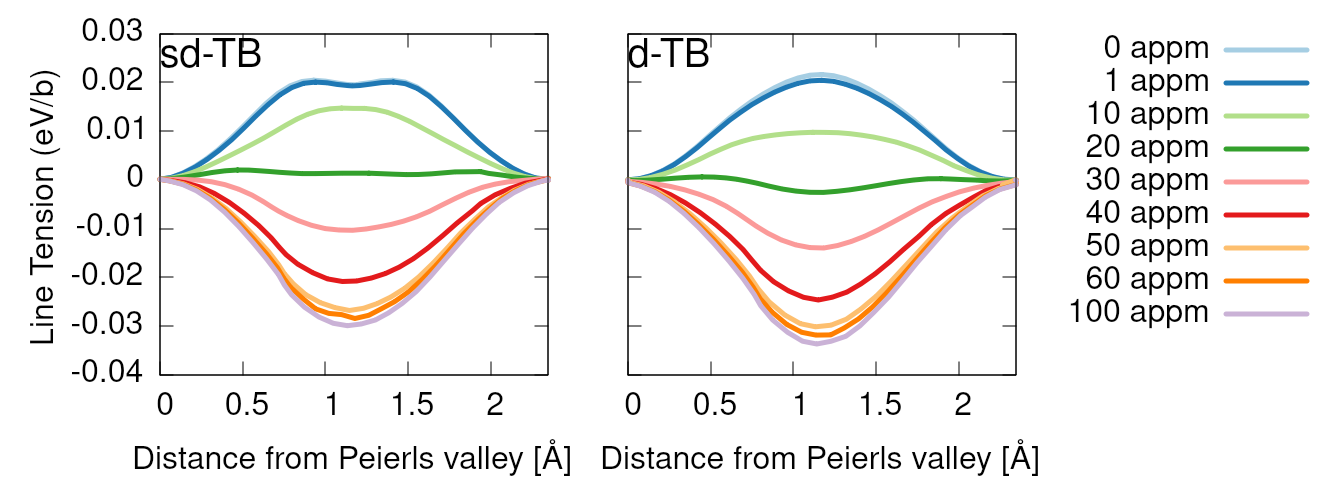
\includegraphics[width=\textwidth]{Images/straight_enthalpies_equib_sdtb_dtb_colorbrewer.png}
    \caption{Enthalpies of straight screw dislocation in the line-tension model in an environment of carbon with concentrations determined by thermodynamical mean field model. Carbon concentration on the dislocation on the dislocation line is in equilibrium with the bulk according to the concentration given by the H1 site, where carbon is able to redistribute between the sites according to Maxwell-Boltzmann statistics.  }
    \label{fig:straighttbequib}
       \end{figure}

    \begin{figure}
\centering
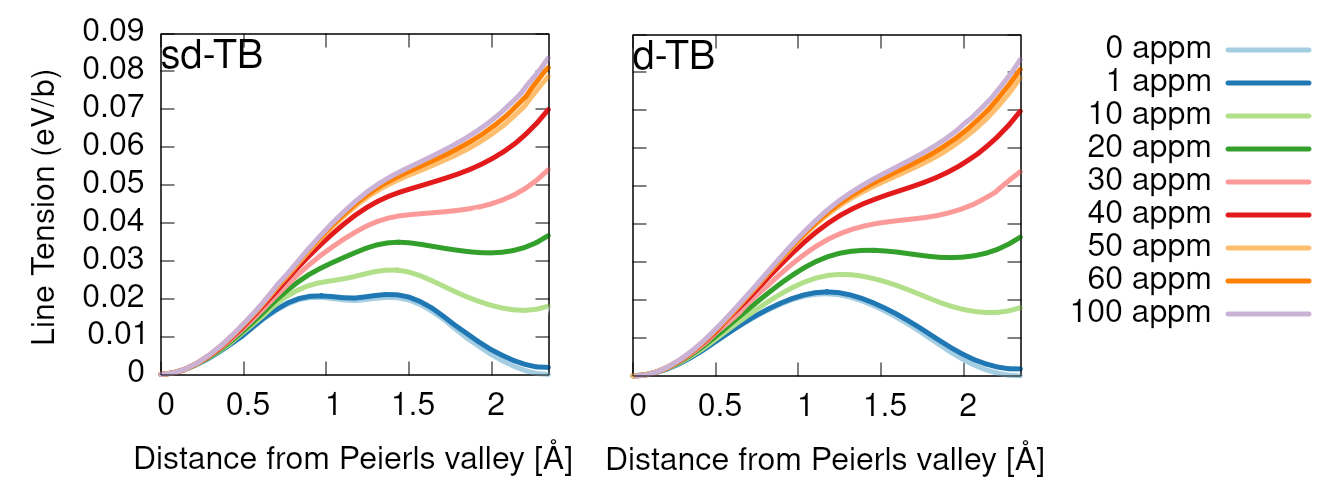
\includegraphics[width=\textwidth]{Images/straight_enthalpies_static_sdtb_dtb_colorbrewer.png}
    \caption{Enthalpies of straight screw dislocation in the line-tension model in an environment of carbon with concentrations determined by thermodynamical mean field model. Concentration of carbon in each of the sites is fixed to its initial value, simulating the limit where carbon does not have time to equlibriate with dislocation movement. }
    \label{fig:straighttbstatic}
       \end{figure}


In equilibrium, the addition of carbon reduces the
peak of the Peierls potential in iron. At 30appm of carbon, the
peak, which was once centered at the hard core position, is now
\emph{below} the reference energy of the easy core state. Dislocations
in easy core will transition to be hard core, with carbon pinning
the dislocation in its prismatic site.

We find that the peak of the peierls potential of the straight
dislocation corresponds to a local minimum
of the peierls potential.

\subsubsection{Dynamics of kink-pair formation in equilibrium}
\label{sec:orgbeb2164}


\begin{figure}[htbp]
\centering
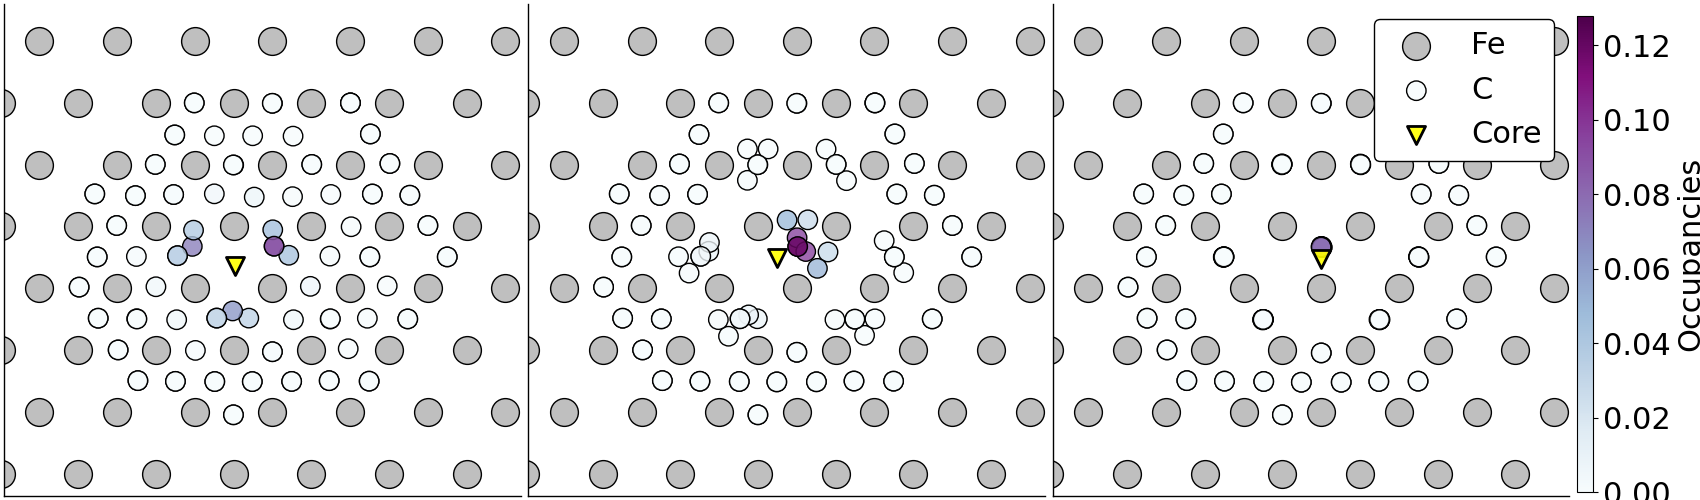
\includegraphics[width=1.\textwidth]{Images/mclean_position_movement_occupancy_forward_alternate.png}
\caption{Positions of trap sites around dislocation segments upon kink-pair formation. Path only shown to the hard core to demonstrate smooth mapping of trap sites going from easy to hard core. Equilibrium occupancies shown by coloured circles.}
\end{figure}

\begin{figure}[htbp]
\centering
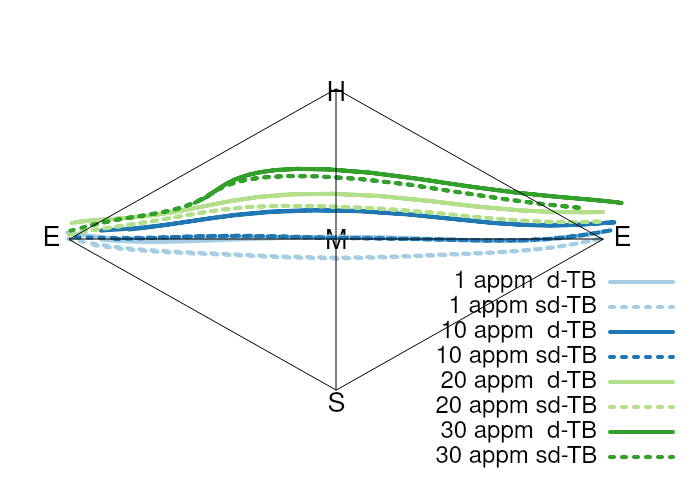
\includegraphics[width=0.8\textwidth]{Images/pathway_equilibrium_sdTB_dTB_30appm.png}
\caption{MEP found upon kink-pair formation in an environment of carbon for both tight-binding models at different nominal carbon concentrations. With an increase in carbon content, path starts to deviate towards more concentrated sites.}
\end{figure}

\begin{figure}[htbp]
\centering
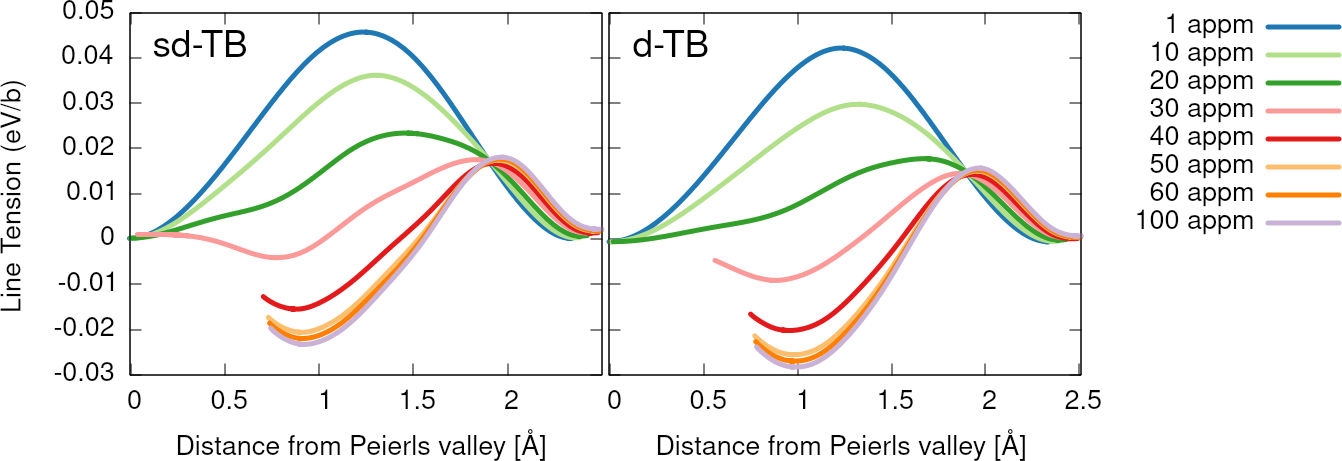
\includegraphics[width=1.\textwidth]{Images/kink-pair_equilibrium_combined_moving_sites.png}
\caption{Positions of trap sites around dislocation segments upon kink-pair formation. Path only shown to the hard core to demonstrate smooth mapping of trap sites going from easy to hard core. Equilibrium occupancies shown by coloured circles.}
\end{figure}

\begin{figure}[htbp]
\centering
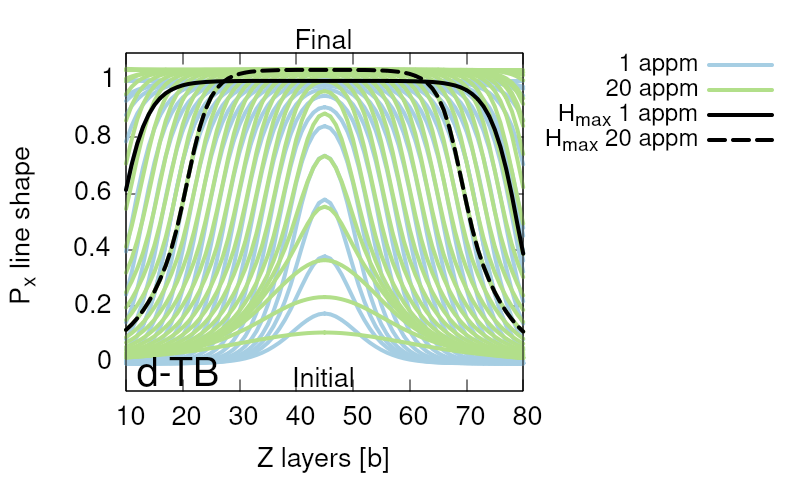
\includegraphics[width=0.9\textwidth]{Images/lineshapes_dtb_moving_sites_labelled18.png}
\caption{\(P_x\) lineshape comparison of differing concentrations of the canonical-\(d\) tight-binding model.}
\end{figure}


\begin{figure}[htbp]
\centering
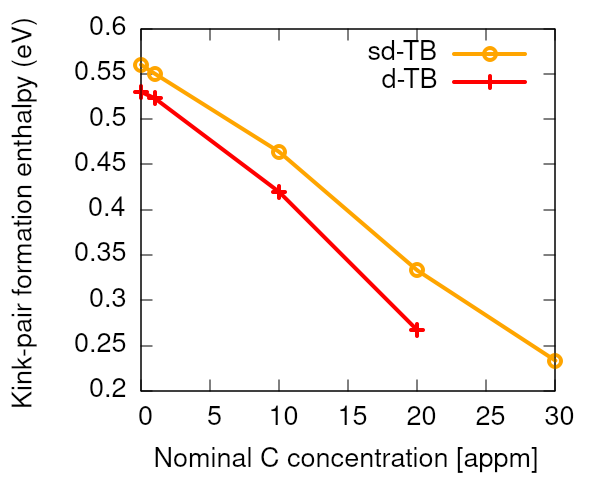
\includegraphics[width=0.7\textwidth]{Images/kink-pair_formation_equilibrium_sdtb_dtb_30appm.png}
\caption{Kink-pair formation enthalpy dependence on nominal carbon concentration.}
\end{figure}

One can assume the slow limit of dislocation movement, and impose
that carbon is in equilibrium with the dislocation.



\section{Discussion}
\label{sec:orgafbdb7e}
\label{sec:discussion}


We expect a reduction in the kink-pair formation enthalpy in tight-binding, due to
the slightly smaller overall Peierls potential along the expected minimum enthalpy
path of the kink within the line tension model. This would increase
the rate of kink nucleation in kMC models, causing a higher overall dislocation
velocity. This will increase the disparity between the dislocation velocity and
the speed of carbon diffusion. In the vicinity of the dislocation line, there is a
"high-mobility" zone for carbon to diffuse easily around the dislocation
\cite{Nematollahi2016}. Assuming a similar kink shape as found in DFT calculations,
we expect the kink-pair formation energy to be \(\sim 0.7\) eV, which similar in
magnitude to the DFT value (\(0.73\) eV) \cite{Itakura2012}. Hence, we predict the
increase in dislocation velocity would not so large as to effectively negate the
effect of the high-mobility zone---which would result in carbon not being able to
"catch-up" to dislocations upon movement. Therefore, we do not expect the observed
discrepancy in the Peierls potential to significantly change the principal
mechanisms observed, or results obtained, from kMC simulations of
dislocation-assisted carbon migration.



As in Lüthi \cite{Lthi2019}, carbon interactions were found to be vital in understanding how screw
dislocations move in steels, due to the spontaneous reconstruction of the pure iron ground state
(easy core) upon introduction of carbon. From the large binding energy of the H1 site, one would
expect a hard core with carbon in a prismatic site as the ground state configuration for pinned
dislocations.

In the context of dislocation-assisted carbon migration, with sufficient contact stress,
dislocations in their hard core ground state will be forced to move (say, along the \(X =
    \langle\bar{2}11\rangle\) direction), which results in the hard core reconstructing to an easy core. Due to
the much higher velocity of dislocations, relative to the diffusivity of carbon, the
prismatic carbon will stay in-place, becoming an E1 site. A drag force now acts to impede motion of the
dislocation, due to the binding of the carbon in the E1 site. Progression of dislocation glide
results in further reconstruction of the dislocation core to hard and easy states, with the
original carbon being situated in H2, E6 and H3 sites, relative to the dislocation
centre. Thus as the dislocation moves, there is a significant drag force acting on the
dislocation, which decreases the further the dislocation moves from carbon, as one would
expect. This suggests that a dislocation-assisted carbon migration mechanism could be feasible,
but the last two stages of the multi-scale model are necessary to verify this.


In normal operating temperatures of the bearing, one expects all dislocations to be hard cores
saturated with carbon (neglecting C-C interaction) in most of the \(\text{H}j\) sites, as seen in
the concentration analysis. In ferrite that has just transformed, assuming a C concentration of
0.6 wt\% as seen in martensite, we expect similar behaviour to the 1000 appm case as seen in
figure \ref{cdhardeasy}. Including C-C interactions would reduce these concentrations from
saturation. There is insufficient data to say how strong this effect would be.



\section{Future work}
\label{sec:org17b1587}

The prerequisites for a line tension model are in place for determination of the kink-pair
formation enthalpies of screw dislocations as a function of carbon content and stress. This is
ongoing work. Validation tests will be carried out on the Itakura data set for the binding of
hydrogen to screw dislocations in bcc iron.


Using the kink-pair formation enthalpies and the binding energies of carbon to screw dislocations, one can proceed
with kinetic Monte Carlo simulation of dislocation glide, in an environment of carbon to
understand how dislocations move carbon under applied stress, in different temperature
and nominal carbon concentration regimes.


It would be of interest to pursue atomistic calculations of carbon bound to edge
dislocations. Recent DFT/Eshelby theory calculations by Maugis \emph{et al.} \cite{Maugis2020}, show
under \emph{compressive} stress, carbon diffusivity is \emph{enhanced}. Pipe diffusion along edge
dislocations could therefore be an important aspect to consider in carbon transport, in addition
to the higher mobility of edge dislocations in bcc iron. As such, edge dislocations could be quite
important within the mechanism of dislocation-assisted carbon migration.

Ising and Monte Carlo models of intersite carbon interactions have been performed using the
results of DFT carbon-dislocation binding energies \cite{Lthi2019}.  These calculations only
considered the hard core, with carbon binding sites of the H1 prismatic site and a H2 site, (which
they name \(P\) and \(O^{(4)}\) respectively). First neighbour C-C interactions were taken
into account, both along the dislocation line and between carbon sites. Using the tight-binding
calculations detailed in this report, we can easily apply and extend this analysis to consider more
binding sites around the hard core, and observe stable carbon distributions around the easy core.

Analysis of carbon diffusion barriers around a dislocation are necessary. In a DFT/EAM
study of carbon-supersaturated ferrite in pearlitic wires, it was found that carbon can diffuse
easily around the dislocation, which is an important consideration in the drag mechanism proposed
\cite{Nematollahi2016}.

\section{Conclusion}
\label{sec:org5b3394f}

Dislocation-assisted carbon migration is thought to be a viable mechanism by which martensite
decays to form DER regions---mostly composed of ferrite interspersed in a martensitic
matrix---which enhances failure risk by RCF. There is dispute over where excess carbon from the
martensitic matrix finds itself upon transformation to ferrite, of much lower carbon
solubility. The current leading mechanism suggests carbon segregates to pre-existing carbides, yet
experimental results show in the late stages of DER formation, pre-existing carbides are partially
dissolved in areas of highly localized plasticity, implying segregation of carbon to
dislocations. As such, a thorough investigation of carbon-dislocation interactions is vital to
understanding how DER initially forms and progresses.

Atomistic calculations using tight-binding, the first stage in a multi-scale paradigm to
understand dislocation-assisted carbon migration, found a Peierls potential with characteristics
comparable to both EAM/DFT results. A canonical \(d\text{-band}\) model may better describe this
energy landscape. It is not expected that the discrepancy in the Peierls potential would
significantly change results in kMC simulations.

Carbon distribution around the easy and hard cores were found to differ
significantly, with the largest binding energy being found by carbon being situated in a prismatic
site in the hard core. Carbon within 3\AA{} of the easy core caused reconstruction to the hard core,
with carbon in a prismatic site.

Equilibrium concentrations of carbon around the hard/easy cores at normal operating temperatures
suggest that all dislocations are of hard core type with carbon situated in a H1/prismatic site, with
reconstruction of all easy core dislocations to hard core, resulting in all dislocations being
pinned.

If a dislocation moves under stress from the hard core-prismatic carbon ground state, a large drag
force acts on the dislocation upon movement to adjacent easy and hard positions, assuming the carbon
will stay in place due to its low diffusion coefficient, relative to dislocation velocity. The
carbon-dislocation binding energies decrease with distance, and are in good agreement with
literature. This suggests that a dislocation-assisted carbon migration mechanism is plausible, but
more work needs to be done to confirm if so.

Further work will be done to ascertain diffusion barriers around the dislocation, which have been
shown to be significantly reduced from bulk values due to the presence of dislocations in DFT/EAM
calculations \cite{Nematollahi2016}. This will complete the description of the solute drag mechanism.

Line tension and kMC models will be used to determine how dislocation glide is affected by carbon
and how carbon can move with dislocations. 


\section{Appendix}
\label{sec:orgfaa7b95}
\subsection{Regularisation of interaction energy in quadrupolar array}
\label{sec:org4cbcd50}
\label{sec:Ainteractionenergy}


In isotropic elasticity, the elastic energy of a single dislocation dipole in an
infinite lattice is given by


\[ E_{\text{el}}^{\infty} = \frac{\mu b^2}{4\pi} ln \big( \frac{r}{r_{c}} \big)  \]

The contribution from periodic images to the correction is 

\[ E_{\text{img} } = E_{\text{el}} (\mathbf{a}, \mathbf{c}_i , r_c) - E_{\text{el}}^{\infty}
   (\mathbf{a}, r_c),\]

"Ghost" dipoles are introduced to account for the conditional convergence of the sum at \(\pm\alpha
   \mathbf{b}\) and \(\pm \beta\mathbf{b}\), where \(\alpha = \beta = 0.5\). We define \(E_{\text{dg}} (\mathbf{R})\) as the
interaction energy of a ghost dislocation and a dipole at \(\mathbf{R}\) anisotropic elasticity
equations as shown in \cite{Cai2003}.


Defining, 
 \[ E_{\text{dd}} (\mathbf{R}) = \frac{\mu b^2}{2\pi}
   \text{ln}\frac{|\mathbf{R}|^2}{|\mathbf{R}+\mathbf{a}|\cdot|\mathbf{R}-\mathbf{a}|},
   \]
we obtain,
\[ E_{\text{img}} = \frac{1}{2}\sum_{\mathbf{R}} [ E_{\text{dd}} (\mathbf{R}) - E_{\text{dg}} (\mathbf{R}) ] - \frac{1}{2}
   E_{\text{dg}} (\mathbf{R} = 0),  \]

which can be subtracted from the total energy as given from atomistic calculations, for a
regularised interaction energy. 


\subsection{Zero-point energy calculation}
\label{sec:org4a447c5}
\label{sec:zeropointenergy}

After relaxation of the C-dislocation system, a 3x3 Hessian matrix is constructed by taking the
numerical derivative of forces observed on the carbon atom after displacement by \(\pm 0.015 \AA\) in
each of the \(X\), \(Y\) and \(Z\) directions.  The three atoms surrounding the core on the first and
third layers were again fixed in \(Z\) coordinate. The zero-point energy is given by

\[ E_z = \frac{1}{2} \sum_{i=1}^3 \frac{h}{2\pi} \sqrt{ k_i /
   m_{\text{C}} },  \]
where \(k_i\) are the eigenvalues of the Hessian and \(m_\text{C}\) is
the mass of carbon. 

\subsection{Smooth mapping of sites in equilibrium line-tension model}
\label{sec:org4159667}
\label{sec:smoothsitemapping}

To approximate the position of trap sites upon dislocation movement, the
\$x\$-coordinate of the dislocation core position, \(P_x\), was used to obtain the trap
site positions around the core.

Focussing on one half of the the path of a dislocation between peierls
valleys, the segment of a dislocation going between an easy core to hard
core, one can define forward and backwards paths, a dislocation travelling
from the easy core towards the hard core, and vice versa. The trap sites at
the end points are well-defined: when \(P_x = P_x^{\text{easy}} = 0\), the trap
sites are exactly those found upon relaxation of the easy core, similarly,
when \(P_x = P_x^{\text{hard}} = a\sqrt{2} / (2\sqrt{3}) = d\), the trap sites are
those found upon relaxation of the hard core. These positions can be seen in
section \ref{sec:fec_binding}.

One can define trap site mappings for these forward and backwards paths: for an easy
core site to a hard core site, \(E_j^{\alpha} \rightarrow H_k^{\beta}\), and
from hard core to easy core \(H_l^{\gamma} \rightarrow E_m^{\delta}\), where
\(j,k,l,m\) denote a particular trap site position, with labels defined in section \ref{sec:fec_binding} and
\(\alpha,\beta,\gamma,\delta\) are labels which denote which of the six possible sectors the
site belongs to. These six sectors arise from the combination of the
three-fold rotational and reflection symmetry found in the crystal---thus one
need only have the trap sites for one sector and apply the appropriate rotation and/or
reflection to obtain the necessary trap site position at the given endpoint. These mappings are not
symmetric for the forward and backwards paths, \emph{e.g.} are many easy core trap
sites which map to the H1 site, due to its strong binding energy, as found in
atomistic simulations of reconstruction, but, quite clearly, these mappings
cannot be imposed for a dislocation going from hard to easy core.


For a given mapping, one can linearly interpolate between the two positions to give a trap site position for an
intermediate dislocation core.

\[ P^{\text{trap forward}}_{j,k}(P_x) =  (1-\frac{P_x}{d})E_j^{\alpha} +   \frac{P_x}{d}H_k^{\beta},\]
\[ P^{\text{trap backward}}_{l,m}(P_x) =  (1-\frac{P_x}{d})E_m ^{\delta} + \frac{P_x}{d}H_l^{\gamma}.\]

To define trap site mappings for core positions at \(P_x > d\), one need only
swap the forward for the backwards path, due to reflection symmetry about
\(P_x = d\), thus allowing for well defined trap sites for all core positions
between the peierls valleys.

\section{Bibliography}
\label{sec:org8cfef06}
\label{org371ac58}

\bibliographystyle{unsrt}
\bibliography{bibliography/org-refs}
\end{document}
